\documentclass[a4paper,10pt]{book}
\usepackage[centertags]{amsmath}
\usepackage{amscd}
\usepackage{amsthm}
\usepackage{amssymb}
\usepackage{enumerate}
\usepackage{multicol}
\usepackage[english,catalan,spanish]{babel}
\usepackage[all]{xy}
\usepackage{color}
\usepackage{tikz}
\usepackage{indentfirst}
\usepackage[utf8]{inputenc}
\usepackage[T1]{fontenc}
\linespread{1.1}
\setlength{\parskip}{10pt}
\usepackage[twoside,bindingoffset=1cm]{geometry}
\usepackage{lmodern}
\usepackage[x11names, dvipsnames, table]{xcolor}
\definecolor{ubblue}{HTML}{0059A2}
\usepackage[colorlinks=true, linkcolor=black, citecolor=ubblue, urlcolor=ubblue]{hyperref}
\usepackage{cleveref}
\usepackage[protrusion=true,expansion=true]{microtype}
\usepackage{cite}
\usepackage{booktabs}
\usepackage{IEEEtrantools}
\usepackage{subcaption}
\usepackage{enumitem}
\setlist[itemize]{itemsep=4pt, parsep=2pt, topsep=2pt, leftmargin=*}



%% Custom packages


%%%%%%%%%%%%%%%%%%%%%%%%%%%%%%%%%%%%%%%%%%%%%%%%%%%%%%%%%%%%%%%%%%%%%%%%%%%
%%%% local definitions for this paper
%%%%%%%%%%%%%%%%%%%%%%%%%%%%%%%%%%%%%%%%%%%%%%%%%%%%%%%%%%%%%%%%%%%%%%%%%%%


%%%%%%%%%%%%%%%%%%%%%% aix{\`o} pels headings %%%%%%%%%%%%%%%%%%%%%%%%
\usepackage{fancyhdr}
\pagestyle{fancy}
\renewcommand{\chaptermark}[1]{\markboth{#1}{}}
\renewcommand{\sectionmark}[1]{\markright{\thesection\ #1}}
\fancyhf{} \fancyhead[LE,RO]{\bfseries\thepage}
\fancyhead[LO]{\bfseries\rightmark} \fancyhead[RE]{\bfseries\leftmark}

\def\paginaenblanc{\newpage%
\thispagestyle{empty}%
\vspace*{2cm}%
\newpage%
\thispagestyle{empty}%
}


%%%%%%%%%%%%%%%%%%%%%%%%%%%%%%%%%%%%%%%%%%%%%%%%%%%%%%%%%%%%%%%%%%%%%%%%%
% aux commands
%%%%%%%%%%%%%%%%%%%%%%%%%%%%%%%%%%%%%%%%%%%%%%%%%%%%%%%%%%%%%%%%%%%%%%%%%
%==========================================================================
% macros to support private authors' notes
%==========================================================================
\newif\ifprivate
\privatetrue
\def\xbar{\vskip0.09in\hrule\vskip0.06in}
\def\private#1{\ifprivate \xbar {\em #1} \xbar
\else \fi}
\def\huh{\ifprivate ??? \marginpar{\Huge ???}
\else \fi}
\def\???{\ifprivate {\bf {???}} \marginpar{\begin{center}{\Huge {\bf ?}}\end{center}}
\else \fi}
%\def\???{\ifprivate {\bf {???}} \marginpar{{\Huge {\bf ?}}}
%\else \fi}
\marginparsep1mm
\def\nota#1{\ifprivate  $\clubsuit$ \marginpar{\parbox[t]{2.4cm}{\begin{center}\tiny #1\end{center}}}
\else \fi}
\def\comment#1{\ifprivate \marginpar{\parbox[t]{2.4cm}{\begin{center}\tiny #1\end{center}}}
\else \fi}
%\def\nota#1{\ifprivate  $\clubsuit$ \marginpar{\parbox[t]{1.8cm}{\tiny #1}}
%\else \fi}
\def\privateeject{\ifprivate\eject\fi}
%\def\???{{\bf {???}} \marginpar{{\Huge {\bf ?}}} }
%%%%%%%%%%%%%%%%%%%%%%%%%%%%%%%%%%%%%%%%%%%%%%%%%%%%%%%%%%%%%%%%%%%%%%%%%%

%%%%%%%%%%%%%%%%%%%%%%%%%%%%%%%%%%%%%%%%%%%%%%%%%%%%%%%%%%%%%%%%%%%%%%%%
%%%%%%%%%%%%%%%%%%%%%%%%%%%%%%%%%%%%%%%%%%%%%%%%%%%%%%%%%%%%%%%%%%%%%%%%
\begin{document}
\bstctlcite{IEEEexample:BSTcontrol}
\pagestyle{empty}

\begin{titlepage}
	\begin{center}
		\begin{figure}[htb]
			\begin{center}
				
\includegraphics[width=6cm]{assets/ub_color.pdf}
			\end{center}
		\end{figure}
				
		\def\worktitle{Development of an AI-Based Tool for Molecular Subtype Classification of Invasive Ductal Breast Carcinoma Using Mammography}
				
		\textbf{\LARGE Treball final de grau} \\
		\vspace*{.5cm}
		\textbf{\LARGE GRAU D'ENGINYERIA INFORM\`{A}TICA } \\
		\vspace*{.5cm}
		\textbf{\LARGE Facultat de Matem\`atiques i Inform\`atica\\ Universitat de Barcelona} \\
		\vspace*{1.0cm}
		\rule{16cm}{0.1mm}\\
		\begin{Huge}
			\textbf{Evaluation of Transformer-Based Models for Molecular Subtype Classification of Invasive Ductal Breast Carcinoma Using Mammography} \\
		\end{Huge}
		\rule{16cm}{0.1mm}\\
				
		\vspace{1cm}
				
		\begin{flushright}
						
						
			\vspace*{2.5cm}
						
			\hfill
						
			\renewcommand{\arraystretch}{1.5}
			\begin{tabular}{ll}
				\textbf{\small Autor:}       & \textbf{\small David Bland\'on T\'orrez }                             \\
				\textbf{\small Director:}    & \textbf{\small Dr. Oliver D\'iaz Montesdeoca }                        \\
				\textbf{\small Realitzat a:} & \textbf{\small  Departament de Matem\`{a}tiques i  Inform\`{a}tica  } \\
				\textbf{\small Barcelona,}   & \textbf{\small \today }                                               
			\end{tabular}
						
		\end{flushright}
				
	\end{center}
		
\end{titlepage}

%%%%%%%%%%%%%%%%%%%%%%%%%%%%%%%%%%%%%%%%%%%%%%%%%%%%%%%%%%%%%%%%%%%%%%%%%
\newpage
\selectlanguage{english}
\noindent \textbf{\large Abstract}

// TODO

%%%%%%%%%%%%%%%%%%%%%%%%%%%%%%%%%%%%%%%%%%%%%%%%%%%%%%%%%%%%%%%%%%%%%%%%%

%%%%%%%%%%%%%%%%%%%%%%%%%%%%%%%%%%%%%%%%%%%%%%%%%%%%%%%%%%%%%%%%%%%%%%%%%
\newpage
\selectlanguage{spanish}
\noindent \textbf{\large Resumen}

// TODO

%%%%%%%%%%%%%%%%%%%%%%%%%%%%%%%%%%%%%%%%%%%%%%%%%%%%%%%%%%%%%%%%%%%%%%%%%

%%%%%%%%%%%%%%%%%%%%%%%%%%%%%%%%%%%%%%%%%%%%%%%%%%%%%%%%%%%%%%%%%%%%%%%%%
\newpage
\selectlanguage{catalan}
\noindent \textbf{\large Resum}

// TODO

%%%%%%%%%%%%%%%%%%%%%%%%%%%%%%%%%%%%%%%%%%%%%%%%%%%%%%%%%%%%%%%%%%%%%%%%%
\newpage
\selectlanguage{english}
\noindent \textbf{\large Acknowledgements}

// TODO
%%%%%%%%%%%%%%%%%%%%%%%%%%%%%%%%%%%%%%%%%%%%%%%%%%%%%%%%%%%%%%%%%%%%%%%%%
\selectlanguage{english}
\pagenumbering{roman} \setcounter{page}{0}
\let\cleardoublepage\clearpage
\tableofcontents
\newpage \thispagestyle{empty}
%%%%%%%%%%%%%%%%%%%%%%%%%%%%%%%%%%%%%%%%%%%%%%%%%%%%%%%%%%%%%%%%%%%%%%%%%

\listoffigures
\listoftables


\pagestyle{fancy}
\markboth{Introducción}{Introducción}
\newpage \thispagestyle{empty}
%%%%%%%%%%%%%%%%%%%%%%%%%%%%%%%%%%%%%%%%%%%%%%%%%%%%%%%%%%%%%%%%%%%%%%%%%
\mainmatter
\chapter{Introduction}
\section{Problem Context}

Breast cancer is one of the leading causes of mortality among women and the most common cancer type in this population. It is estimated that, on average, one in every twenty women worldwide will be diagnosed with breast cancer during their lifetime \cite{kim_global_2025}. Recent projections suggest that, if the current trend continues, by 2050 there will be approximately 3.2 million new cases and 1.1 million deaths from this disease, with a particularly significant impact in countries with low Human Development Index (HDI) scores \cite{kim_global_2025}.

In this context, early diagnosis and diagnostic imaging tools play a fundamental role in improving patient prognosis and survival \cite{wang_early_2017}. However, breast cancer is a heterogeneous disease\footnote{Cellular diversity present within a tumor (intratumoral heterogeneity) or between different tumors in the same individual (intertumoral heterogeneity).} that can be classified into various subtypes according to clinical and, particularly, molecular characteristics. The 2013 St. Gallen International Consensus Guidelines \cite{goldhirsch_personalizing_2013} defined four main subtypes based on hormone receptors (estrogen and progesterone) and the proliferation marker Ki67: Luminal A, Luminal B, HER2 positive (HER2-enriched), and Triple Negative (see Figure \ref{fig:subtypes}). This classification has direct clinical implications, as prognosis, therapeutic response, and treatment options are largely determined by the molecular subtype of the tumor.

Currently, molecular tumor characterization is mainly performed through tissue biopsy, an invasive and costly procedure that may require repetition, potentially delaying treatment initiation and increasing the clinical, physical, and emotional burden on patients. Therefore, there is a growing need to develop non-invasive, accessible, and efficient methods for reliable molecular subtype classification. In this regard, x-ray mammography stands out as the gold standard imaging modality, as it is a non-invasive, low-cost technique widely utilized for breast cancer screening and diagnosis due to its demonstrated effectiveness in clinical practice.

\begin{figure}
	\centering
	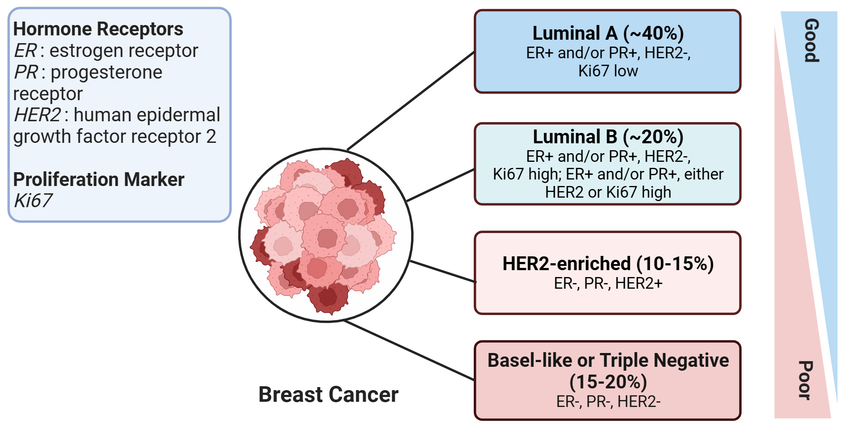
\includegraphics[width=0.8\linewidth]{reports/assets/subtypes.png}
	\caption[Classification of breast cancer molecular subtypes.]{Classification of breast cancer molecular subtypes, showing approximate proportions (\%) among all breast cancer cases. Subtypes are ordered by prognosis severity, with those having better outcomes at the top and progressively worse prognoses toward the bottom \cite{harnessing_2024}.}
	\label{fig:subtypes}
\end{figure}

In recent years, advances in artificial intelligence (AI), together with the increasing availability of data and increasingly powerful computational resources, have driven the development of deep learning (DL) models for breast cancer classification, detection, and prognosis prediction, as well as applications in other diseases. Several studies have demonstrated that these systems can match or even surpass the performance of human experts or CAD\footnote{Computer-Aided Diagnosis} systems in these tasks \cite{mckinney_international_2020,pattanaik_breast_2022,meenalochini_deep_2024,hussain_performance_2025}, highlighting the significant potential of this technology to improve clinical practice and patient outcomes.

Recent research has explored breast cancer molecular subtype classification from mammographic images. For example, Mota et al. (2024) \cite{mota_breast_2024} investigated this challenge, achieving a multi-class area under the curve (AUC)\footnote{A metric used in machine learning to evaluate the performance of classification models.} of 60.62\% using a ResNet-101 architecture. Similarly, Rabah et al. (2025) \cite{ben_rabah_multimodal_2025} obtained an AUC of 61.3\% with a Xception model in unimodal\footnote{Use only one type of data as input (images, text, video, etc.).} settings and developed a multimodal approach integrating clinical metadata, which achieved 88.87\% AUC. While unimodal approaches yield modest performance that remains below clinically acceptable thresholds (~80\% AUC), these studies highlight the diagnostic potential of mammographic imaging and underscore the importance of continued research to improve the accuracy and clinical utility of these models.

This study proposes a unimodal approach based exclusively on the inference based on mammograms from the public CMMD dataset (The Chinese Mammography Database) \cite{cai_online_2023}, comparing the performance of state-of-the-art Transformer architectures including Vision Transformer (ViT), Swin Transformer (Swin), and Multi-Axis Vision Transformer (MaxViT) against a traditional ResNet-101 baseline. While multimodal models typically achieve superior results by integrating complementary clinical data, a unimodal approach focused exclusively on mammographic images offers significant practical advantages, especially in resource-limited settings or when clinical data standardization is unavailable. Recent studies have demonstrated that Transformers-based models outperform convolutional neural networks (CNN) in accuracy and robustness for medical image classification tasks due to their self-attention mechanisms, which enable them to capture global spatial relationships across images \cite{mauricio_comparing_2023}. Based on these architectural advantages, this study hypothesizes that Transformer architectures will achieve superior performance in molecular subtype classification, even under a unimodal approach.

Ultimately, this work seeks to contribute to the development of non-invasive diagnostic tools through systematic evaluation of vision transformer models, advancing automated, accessible, and efficient molecular characterization of breast cancer. This approach is particularly valuable in clinical scenarios where tissue biopsy is not immediately feasible, potentially improving diagnostic equity and reducing time to treatment initiation.


\section{Planning}

\subsection{Objectives}

The \textbf{primary objective} of this study is to systematically compare vision Transformer architectures against a CNN baseline for mammography-based molecular subtype classification, establishing performance benchmarks for non-invasive breast cancer characterization.

To achieve this primary objective, the following \textbf{secondary objectives} are proposed:

\begin{enumerate}
	\item \textbf{Conduct a comprehensive literature review} of AI approaches for breast cancer molecular subtype classification, analyzing current research and performance benchmarks.
	\item \textbf{Identify and address dataset challenges} through appropriate preprocessing strategies, including class imbalance mitigation via weighted loss functions, balanced sampling techniques, and data augmentation methods.
	\item \textbf{Develop and implement} a robust stratified k-fold cross-validation framework for training and evaluating Vision Transformer architectures (ViT, Swin Transformer, and MaxViT) on mammographic images.
	\item \textbf{Establish comparative performance analysis} against a ResNet-101 baseline and benchmark results from existing literature using standardized evaluation metrics (Accuracy, AUC, F1-Score, Precision, Recall, Cohen-Kappa).
	\item \textbf{Perform statistical validation} of model performance differences through statistical tests to ensure result significance and reliability.
	\item \textbf{Apply interpretability analysis} using Grad-CAM and attention visualization techniques to identify mammographic features most relevant to molecular subtype discrimination.
	\item \textbf{Synthesize findings and provide recommendations} for future research directions and clinical implementation considerations.
\end{enumerate}

\subsection{Tasks to Develop}

In order to address the aforementioned objectives of the project, several tasks have been identified, as described below. 

\textbf{State of the Art}

\begin{enumerate}
	\item \textbf{Medical context}: Review current scientific literature on breast cancer to contextualize its clinical and epidemiological relevance.
	\item \textbf{Problem intuition}: Analyze the importance of molecular characterization in breast cancer, highlighting its advantages, limitations, and current challenges.
	\item \textbf{Previous works}: Examine recent advances in AI and deep learning for breast cancer characterization and diagnosis, comparing approaches and results reported in the literature.
\end{enumerate}

\textbf{Implementation}

\begin{enumerate}
	\item \textbf{Data Collection}: Acquire images and familiarize with the dataset's structure, organization, and provided metadata.
	\item \textbf{Data Analysis and Preprocessing}: Analyze class distribution, data consistency, and perform image preprocessing.
	\item \textbf{Project Coding}: Develop code to conduct experiments, train, and evaluate the different models.
	\item \textbf{Result Analysis}: Evaluate and interpret results to draw conclusions and propose future work.
\end{enumerate}

\textbf{Report Preparation}

\begin{enumerate}
	\item \textbf{Report Writing}: Document all procedures, including methodology, materials, results, and conclusions.
	\item \textbf{Revisions}: Incorporate feedback from advisor and refine until achieving acceptable quality.
	\item \textbf{Submission and Presentation}: Submit the thesis and prepare a summary of key findings for the committee presentation.
\end{enumerate}

\subsection{Planning}

The project planning is represented in the Gantt chart below (Figure \ref{fig:roadmap}), outlining previously defined tasks across the 4 months of the project (Spring Semester).

\begin{figure}[h!]
	\centering
	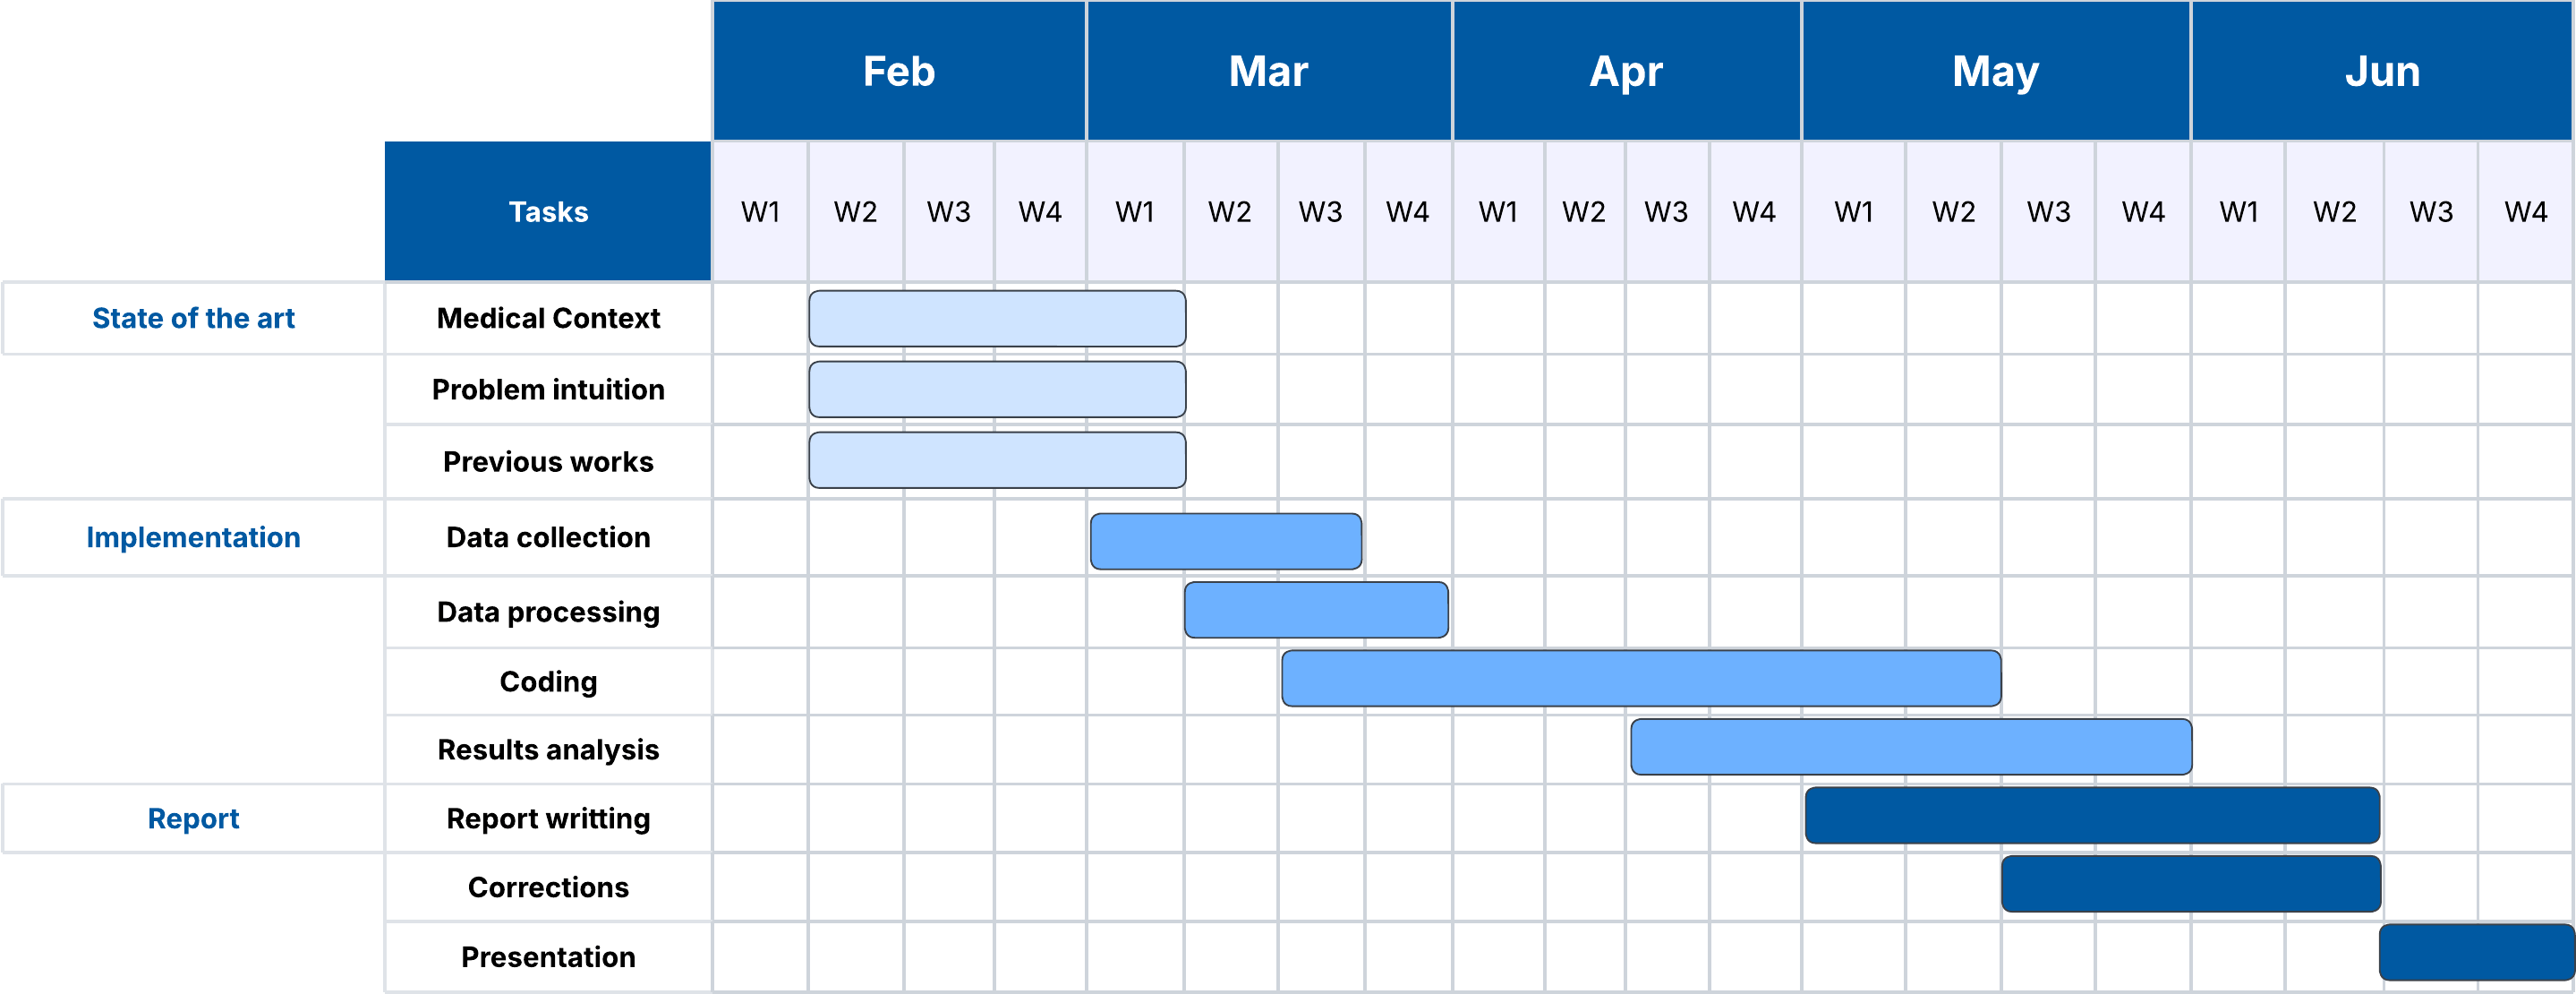
\includegraphics[width=1\linewidth]{reports//assets/RoadmapV3.png}
	\caption[Planning Gantt Chart]{Gantt Chart.}
	\label{fig:roadmap}
\end{figure}

%%%%%%%%%%%%%%%%%%%%%%%%%%%%%%%%%%%%%%%%%%%%%%%%%%%%%%%%%%%%%%%%%%%%%%%%%

\chapter{Background}

\section{Breast Cancer}

Breast cancer is a malignant neoplasm\footnote{An abnormal and uncontrolled growth of cells that gives rise to a mass or tumor, called benign if it grows slowly and remains localized, or malignant if it is invasive and fast-growing.} that originates in the glandular tissue of the breast, mainly in the ducts and lobules, where certain cells undergo genetic mutations that disrupt their growth control. 

These alterations allow cells to multiply uncontrollably, forming tumor masses that can infiltrate adjacent tissues and even spread to distant organs through the lymphatic system and bloodstream. In the absence of early diagnosis and timely treatment, this spread, also known as metastasis, can seriously compromise patient survival. Figure \ref{fig:breast-cancer-anatomy} illustrates the anatomical structure of the breast, showing how tumors develop within normal breast tissue.

\begin{figure}[h]
	\centering
	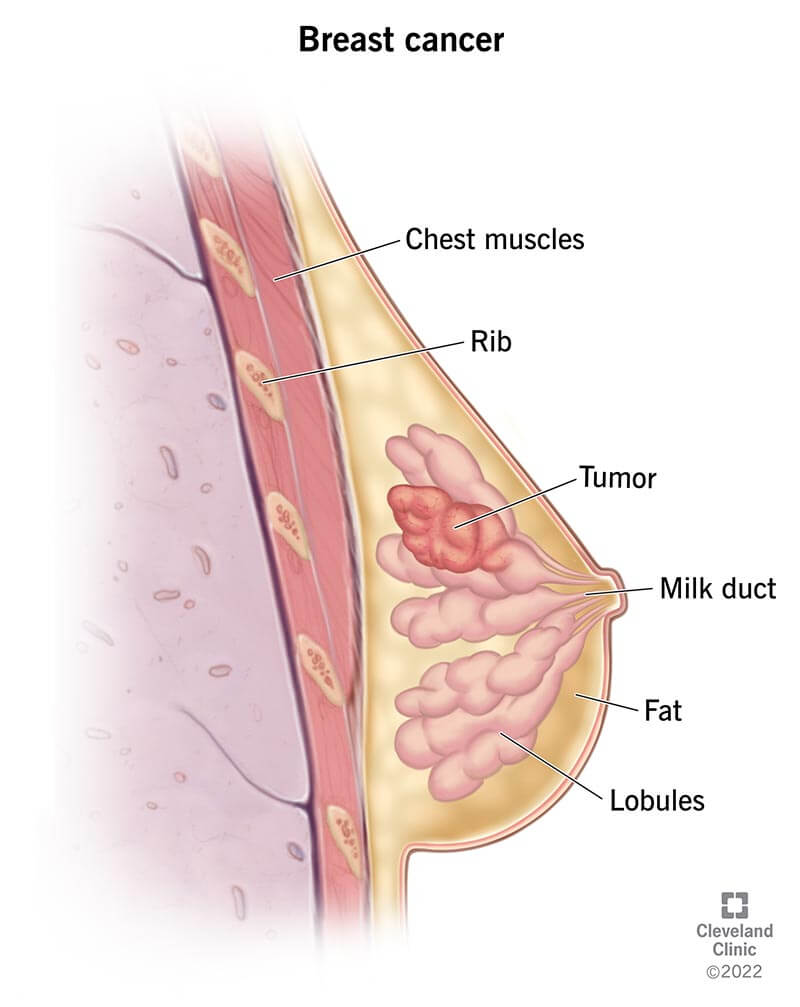
\includegraphics[width=0.3\linewidth]{reports//assets/bc.jpg}
	\caption[Anatomy of breast cancer]{Anatomy of breast cancer \cite{cleveland_clinic_breast_2023}.}
	\label{fig:breast-cancer-anatomy}
\end{figure}

\subsection{Epidemiology}

Globally, it is the most common neoplasm among women and the leading cause of cancer-related mortality in this population. In 2022, approximately 2.3 million new cases were estimated, with 670,000 deaths from this disease, according to the World Health Organization (WHO) \cite{who_breast_2024}. In Spain, breast cancer accounts for nearly 30\% of all cancer cases, and projections from the Spanish Society of Medical Oncology (SEOM) estimate around 37,400 new cases in 2025 \cite{seom_cancer_nodate}.

\subsection{Clinical Classification}

Most breast cancers are carcinomas, which are malignant tumors that originate in the ducts or lobules of the breast. These carcinomas constitute more than 95\% of all breast cancer cases \cite{makki_diversity_2015, noauthor_types_nodate}. From a clinical perspective, these tumors can be classified according to various criteria, among which the following stand out:

\textbf{According to their degree of invasion}
\begin{itemize}
	\item \textbf{Carcinoma in situ}: A tumor in which abnormal cells are confined within the breast ducts and have not crossed the natural barrier separating them from the rest of the breast tissue. Although not invasive, it is considered a precursor lesion and high-risk.
	\item \textbf{Invasive carcinoma}: A tumor that has breached the ducts or lobules of the breast and invaded the surrounding breast tissue. It can spread to lymph nodes or distant sites. 
\end{itemize}

\textbf{According to histological origin}
\begin{itemize}
	\item \textbf{Ductal carcinoma}: Originates in the milk ducts\footnote{Ducts that carry milk from the mammary glands to the nipple.} and is the most common subtype.
	\item \textbf{Lobular carcinoma}: Originates in the breast lobules and tends to show a more diffuse pattern of spread.
\end{itemize}

Figures \ref{fig:histological_types_one} and \ref{fig:histological_types_two} show the differences between ductal and lobular carcinoma, both in situ and invasive.

\begin{figure}[h!]
	\centering
	\begin{subfigure}[c]{0.48\textwidth}
		\centering
		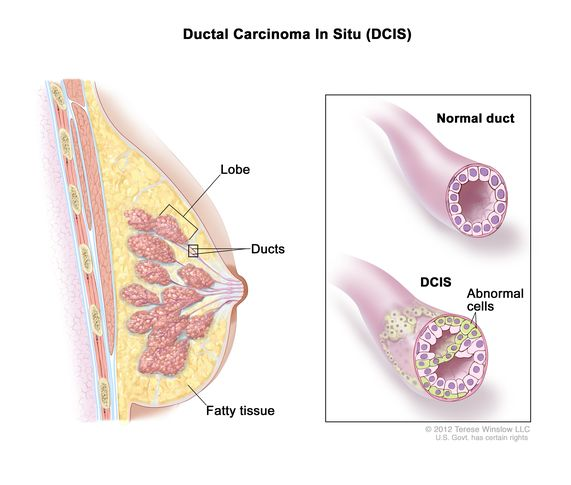
\includegraphics[width=\textwidth]{reports/assets/dcis.jpg}
		\caption{Ductal carcinoma in situ}
		\label{fig:dcis}
	\end{subfigure}
	\begin{subfigure}[c]{0.48\textwidth}
		\centering
		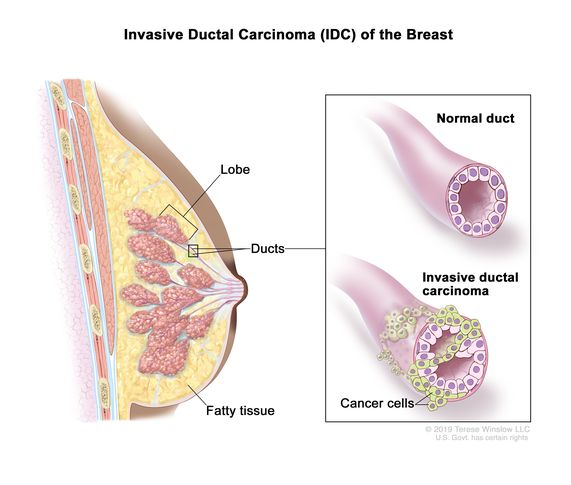
\includegraphics[width=\textwidth]{reports/assets/idc.jpg}
		\caption{Invasive ductal carcinoma}
		\label{fig:idc}
	\end{subfigure}
	\caption[DCIS vs. IDC comparison]{Anatomical comparison between ductal carcinoma in situ (DCIS) and invasive ductal carcinoma (IDC). (a) DCIS shows abnormal cells confined within the milk duct structure, while (b) IDC demonstrates cancer cells that have broken through the duct wall and invaded surrounding breast tissue \cite{noauthor_nci_2011}.}
	\label{fig:histological_types_one}
\end{figure}

\begin{figure}[h!]
	\centering
	\begin{subfigure}[c]{0.48\textwidth}
		\centering
		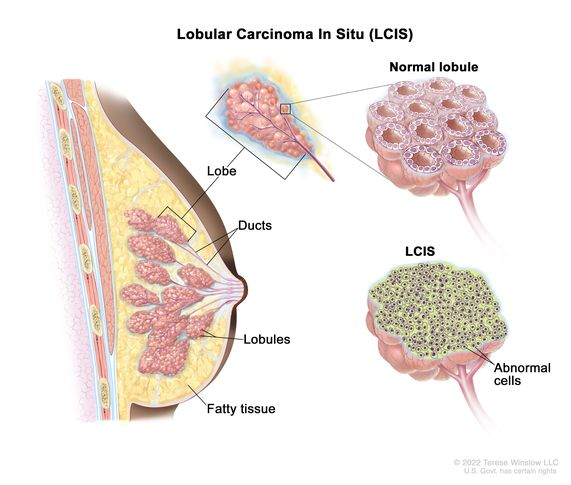
\includegraphics[width=\textwidth]{reports/assets/lcis.jpg}
		\caption{Lobular carcinoma in situ}
		\label{fig:lcis}
	\end{subfigure}
	\begin{subfigure}[c]{0.48\textwidth}
		\centering
		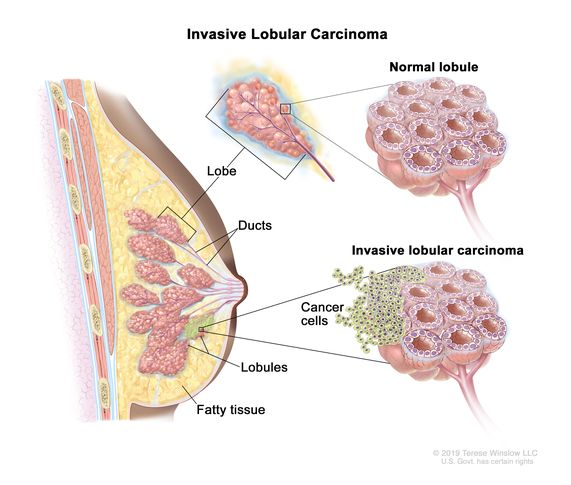
\includegraphics[width=\textwidth]{reports/assets/ilc.jpg}
		\caption{Invasive lobular carcinoma}
		\label{fig:ilc}
	\end{subfigure}
	\caption[LCIS vs. ILC comparison]{Progression from lobular carcinoma in situ (LCIS) to invasive lobular carcinoma (ILC). (a) LCIS represents abnormal cell growth restricted to the milk-producing lobules, whereas (b) ILC shows malignant cells spreading from lobules into adjacent breast tissue \cite{noauthor_nci_2011}.}
\label{fig:histological_types_two}
\end{figure}

\textbf{According to staging systems}

Clinical staging systems are a way of determining how much cancer there is and how far it has spread in the body, using tests and assessments done before surgery or other treatment. This provides standardized frameworks for prognosis and treatment planning.

\begin{itemize}
	\item \textbf{BI-RADS Staging System}: The Breast Imaging-Reporting and Data System (BI-RADS)\cite{magny_breast_2025} standardizes mammographic interpretation and assigns suspicion categories that guide medical management (see Table \ref{tab:birads_table}).
    \item  \textbf{TNM Staging System}: This is the most widely used staging system \cite{noauthor_stages_nodate}. It evaluates three key anatomical factors:
    \begin{itemize}
        \item \textbf{Tumor(T)}: Size and local extent of the primary tumor, ranging from TX (tumor cannot be assessed) to T4 (extensive local invasion).
        \item \textbf{Node(N)}: Regional lymph node involvement, from NX (nearby lymph nodes cannot be assessed) to N3 (extensive nodal spread).
        \item \textbf{Metastasis(M)}: Presence or absence of distant metastases (M0 or M1).
  \end{itemize}
  The current TNM system, updated in 2018, incorporates new parameters like estrogen receptor (ER), progesterone receptor (PR), and others clinical variables to provide more accurate prognostic stratification \cite{hortobagyi_new_2018}. 
  
\end{itemize}

\begin{table}[h!]
	\caption[Breast Imaging-Reporting and Data System (BI-RADS)]{Breast Imaging-Reporting and Data System (BI-RADS) classification \cite{noauthor_bi-rads_2025}.}
	\centering
	\begin{tabular}{lccccc}
		\toprule
		\textbf{Category} & \textbf{Definition} & \textbf{Likelihood of cancer}\\
		\midrule
		BI-RADS 0        & Incomplete                         & N/A \\
		BI-RADS 1        & Negative                           & Essentially 0\% \\
            BI-RADS 2        & Benign                             & Essentially 0\%  \\
            BI-RADS 3        & Probably benign                    & > 0\% but $\leq 2\%$ \\
            BI-RADS 4        & Suspicious                         & > 2\% but < 95 \% \\
            BI-RADS 5        & Highly suggestive of malignancy    & $\geq 95\%$ \\
            BI-RADS 6        & Known biopsy-proven malignancy     & N/A \\
		\bottomrule
	\end{tabular}
	\label{tab:birads_table}
\end{table}


In addition to these classifications, in recent years, molecular subtyping of breast cancer, based on biomarker expression and genomic profiles, has gained particular relevance, which will be addressed in the next section.


\subsection{Molecular Subtypes}

Although clinical and histological classification of breast cancer provides important information for diagnosis, it does not always allow for precise prediction of the tumor’s biological behavior or its response to specific treatments.

The research by Perou et al. (2000) \cite{perou_molecular_2000} and Sørli et al. (2003) \cite{sorlie_repeated_2003} laid the groundwork for the molecular characterization of breast cancer. Through gene expression profiling\footnote{A study that identifies which genes are active and to what extent in a cell or tissue by analyzing RNA levels produced by thousands of genes simultaneously.}, Perou et al. demonstrated that breast cancer is a heterogeneous disease and proposed a molecular subtype classification based on the genetic expression patterns of the tumors analyzed. Four subtypes were initially defined: \textbf{Luminal A}, \textbf{Luminal B}, \textbf{HER2}, and \textbf{Basal-like (Triple negative)}.

Sørli et al. reinforced these findings. They replicated the research in different patient cohorts, demonstrating that the results were not artifacts of a single study. They also showed that molecular subtypes are associated with clinically significant differences, such as prognosis and risk of distant metastasis, giving this characterization greater predictive value than traditional histological classification.

\begin{figure}
	\centering
	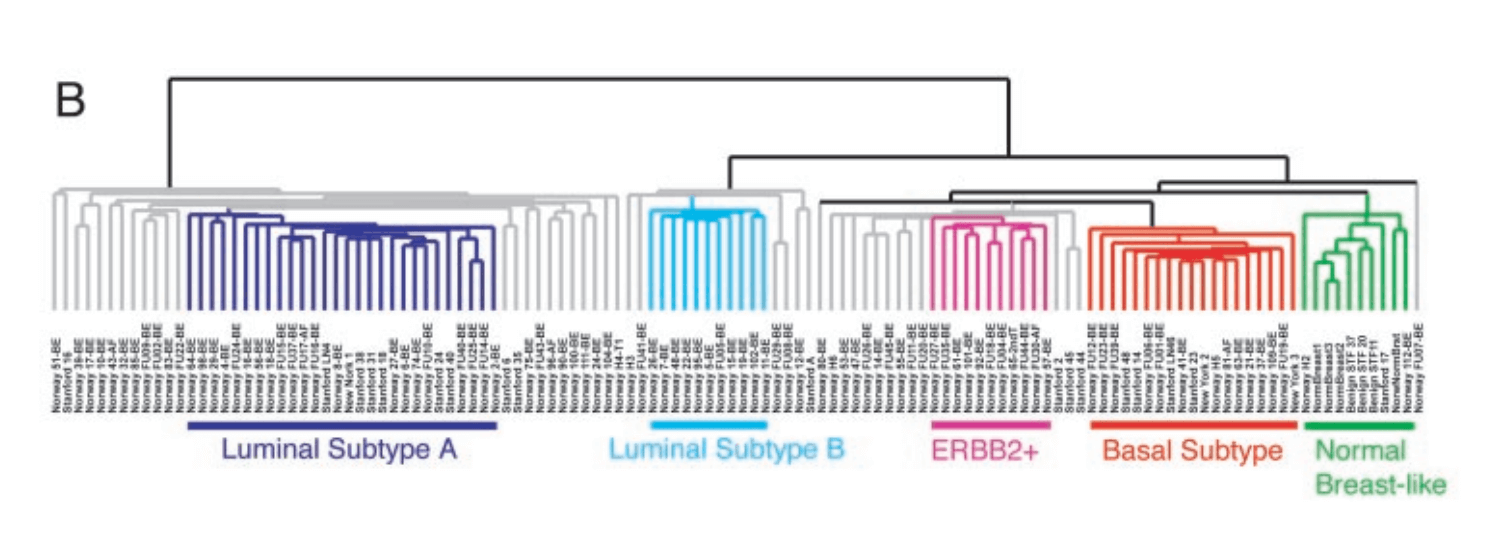
\includegraphics[width=0.8\linewidth]{reports//assets/dendogram.png}
	\caption[Molecular subtypes dendrogram by Sørli et al.]{Dendrogram from the study by Sørli et al. showing the clustering of subtypes according to genetic patterns \cite{sorlie_repeated_2003}.}
	\label{fig:sorlie-dandrogram}
\end{figure}

Following these studies, efforts focused on translating the findings into clinical practice. Since the technique used for classification at the time (DNA microarrays) was expensive, complex, and not accessible to most hospitals, an alternative was sought. It was at the St. Gallen international consensus meetings that classification criteria based on immunohistochemical (IHC) markers were proposed, formalizing the subtypes using a combination of the following hormone receptors \cite{lips_breast_2013}:

\begin{itemize}
	\item \textbf{Estrogen (ER) and Progesterone (PR) Receptors}: Define the tumor’s hormonal dependence, which can affect its growth. Tumors with these receptors respond well to hormonal therapy.
	\item \textbf{HER2 (Human epidermal growth factor receptor 2)}: A protein that stimulates cell growth. Its overexpression usually indicates a more aggressive subtype.
	\item \textbf{Ki-67}: The cell proliferation index. High Ki-67 suggests a more aggressive and rapidly proliferating tumor.
\end{itemize}

Table \ref{tab:molecular_subtypes_comb} shows these classification criteria.

\begin{table}[h!]
	\centering
        \caption[Breast cancer molecular subtypes classification criteria]{Classification criteria for molecular subtypes from the St. Gallen 2013 consensus \cite{goldhirsch_personalizing_2013}}.
	\begin{tabular}{lccccc}
		\toprule
		\textbf{Subtype} & \textbf{HER2} & \textbf{ER} & \textbf{PR} & \textbf{Ki-67} \\
		\midrule
		Luminal A        & Negative      & Positive    & Positive    & < 14\%         \\
		Luminal B/HER2-  & Negative      & Positive    & -           & $\geq$ 14\%    \\
		Luminal B/HER2+  & Positive      & Positive    & -           & -              \\
		HER2-enriched    & Positive      & Negative    & Negative    & -              \\
		Triple Negative  & Negative      & Negative    & Negative    & -              \\
		\bottomrule
	\end{tabular}
	\label{tab:molecular_subtypes_comb}
\end{table}

The Luminal A subtype is the most frequent, representing 70\% of cases at diagnosis. These tumors are characterized by slower growth and respond well to hormonal therapies, making them tumors with a better prognosis and higher survival rates. Luminal B tumors are more aggressive, have a more guarded prognosis, and are more likely to recur. They tend to be more resistant to hormonal treatments and may require chemotherapy.

HER2-enriched tumors account for 10–15\% of cases, distinguished by a rapid growth rate and overexpression of HER2, without hormone receptors. Finally, the triple negative subtype, also appearing in 10–15\% of diagnoses, lacks expression of ER, PR, and HER2. This group displays more aggressive clinical behavior, with a high rate of early recurrence and limited therapeutic options, as it does not respond to hormone therapy or targeted treatments. Conventional chemotherapy is currently the main therapeutic strategy.

\section{Medical Imaging}

Medical imaging encompasses a set of techniques and procedures used to generate visual representations of the interior of the human body for clinical and scientific purposes. These tools enable non-invasive visualization of anatomical structures and physiological processes, facilitating disease diagnosis and the study of normal and pathological anatomy.

For breast cancer diagnosis, several imaging techniques are currently employed, each with specific advantages and limitations depending on patient characteristics and clinical context, as shown in Figure \ref{fig:breast_cancer_medical}.

\begin{figure}[h!]
    \centering
    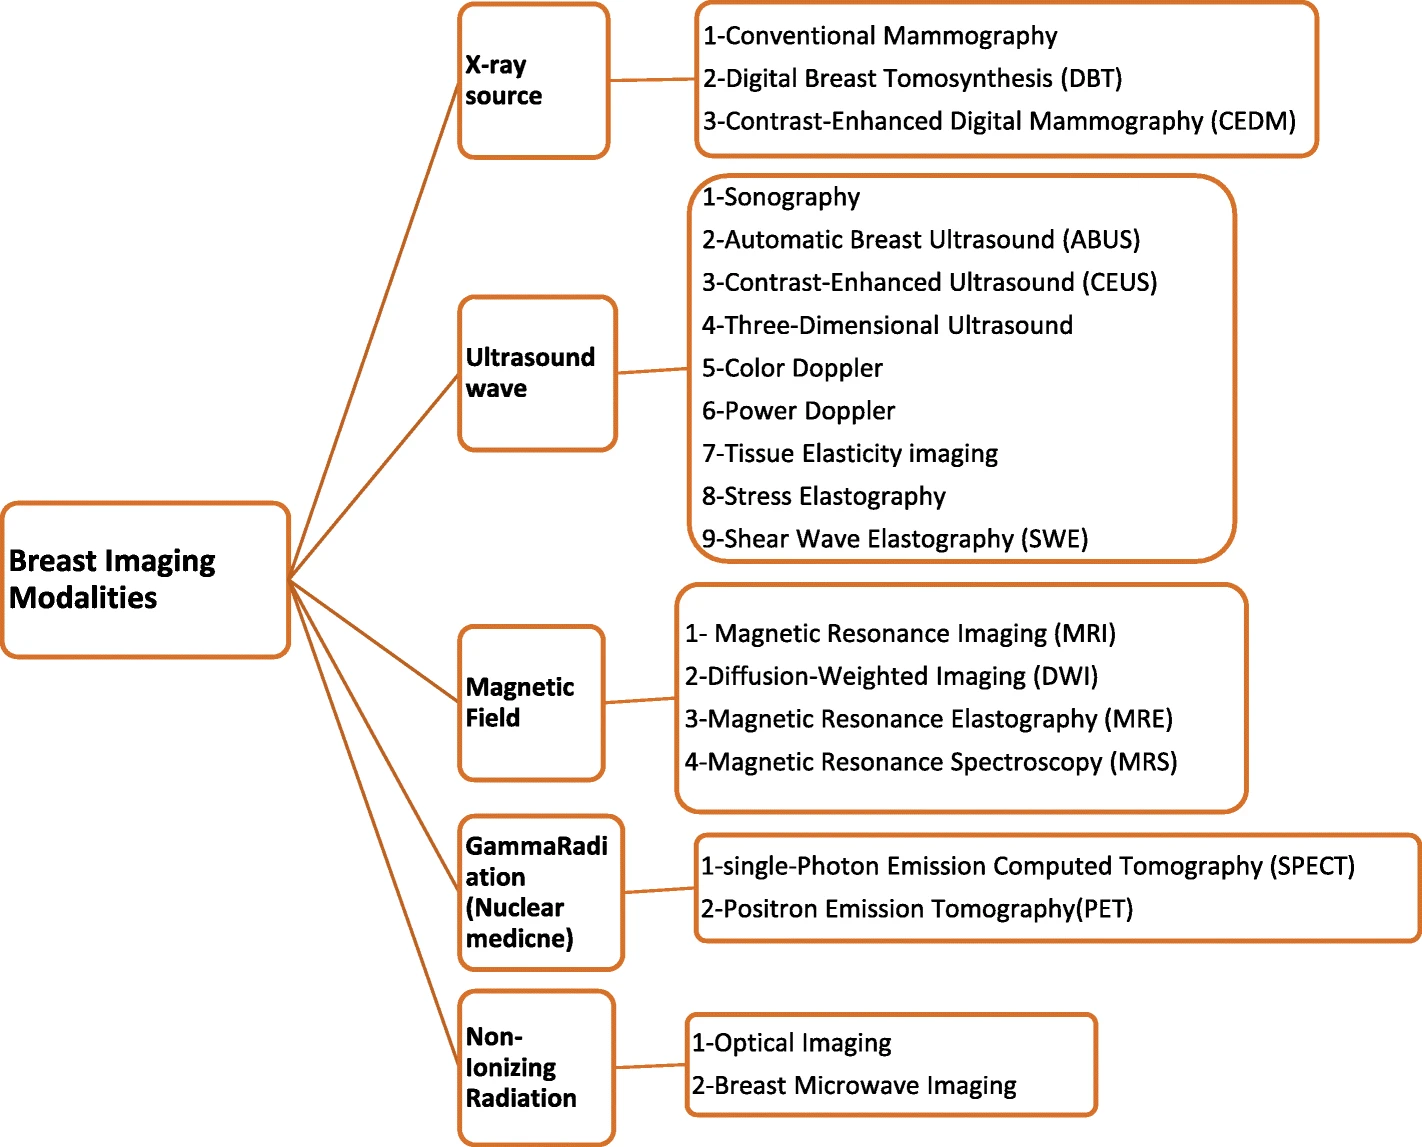
\includegraphics[width=0.75\linewidth]{reports//assets/medical_imaging.png}
    \caption[Overview of breast imaging modalities]{Overview of breast imaging modalities classified by the type of physical principle used, including x-ray, ultrasound, magnetic field, gamma radiation and non-ionizing techniques \cite{iranmakani_review_2020}.}
    \label{fig:breast_cancer_medical}
\end{figure}

\subsection{X-ray Mammography}

In this work, X-ray mammography images will be used as input to our model to infer the molecular subtype of breast cancer. As the standard imaging technique in population-based screening programs, X-ray mammography was specifically developed to examine the breast and other soft tissues. The procedure is performed using a specialized medical imaging device known as a mammography unit or mammography machine. During the exam, the breast is positioned on a flat support plate and gently compressed with a paddle. A brief burst of X-rays is then passed through the breast to a detector on the opposite side, which captures detailed images for analysis (Figure \ref{fig:mammography}).

\begin{figure}[h!]
    \centering
    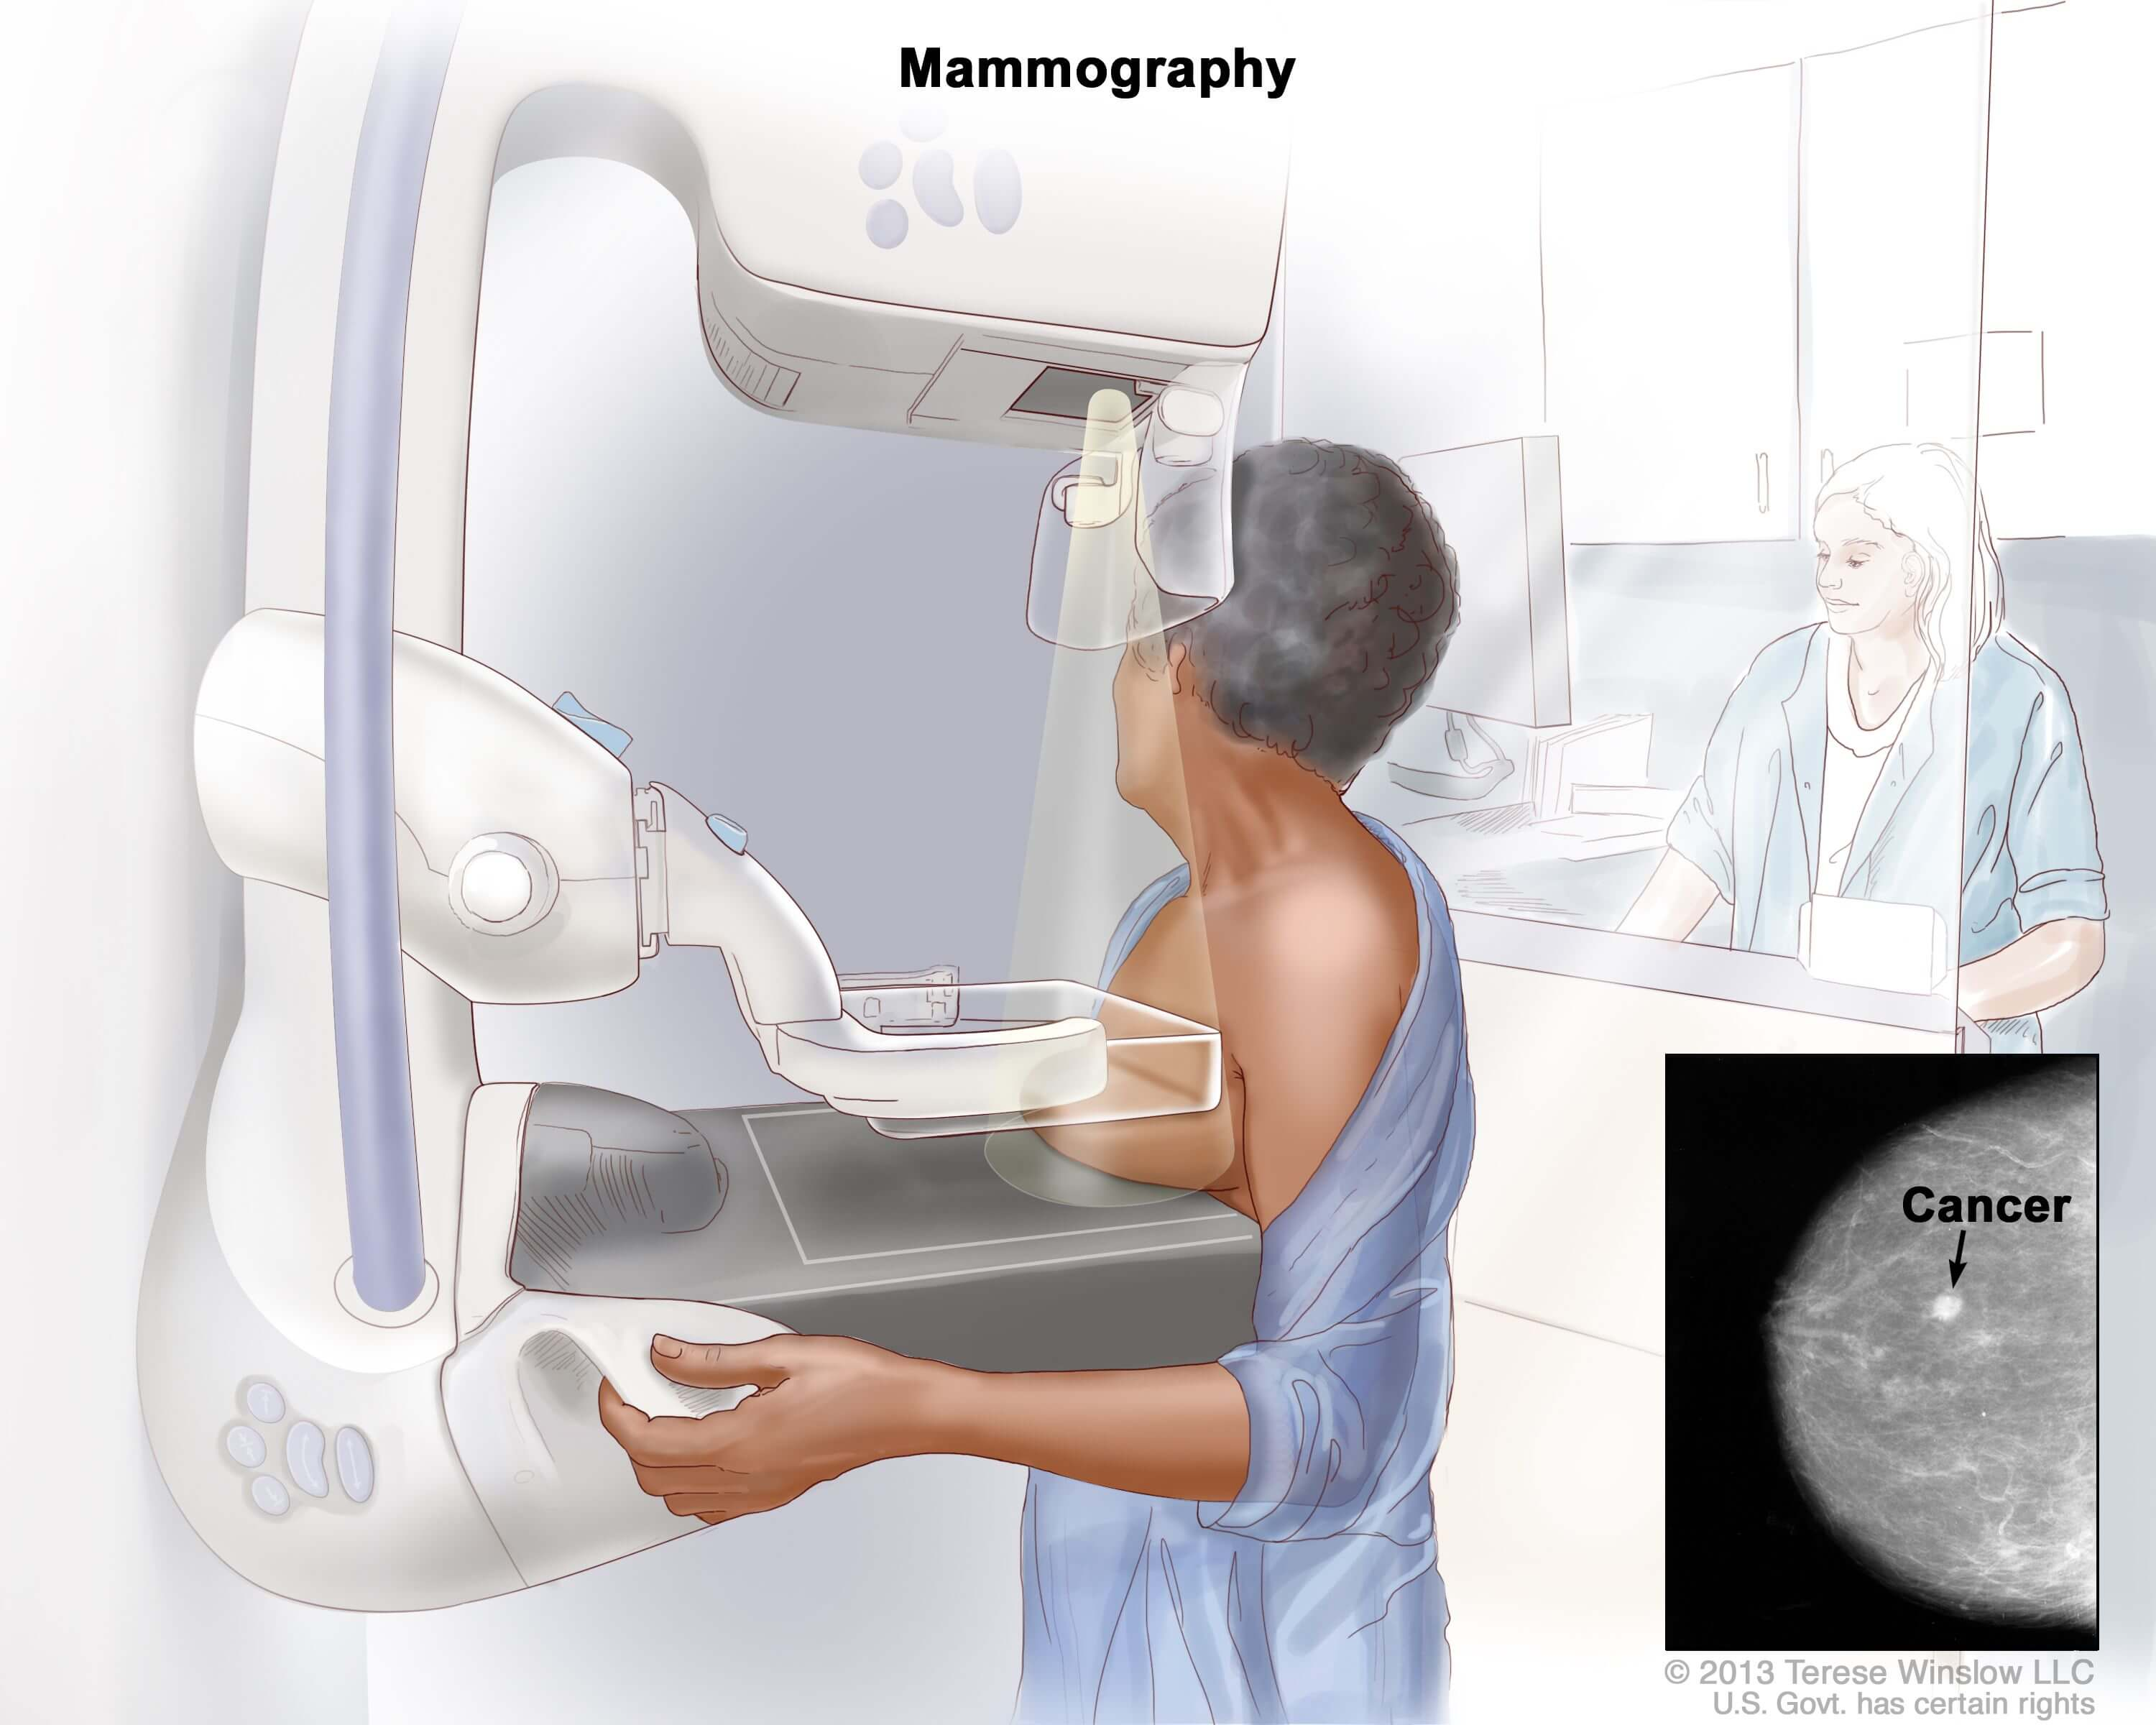
\includegraphics[width=0.45\linewidth]{reports//assets/mammography.jpg}
    \caption[Traditional mammography procedure]{Illustration showing the traditional mammography procedure \cite{nihDefinitionMammogramNCI2011}.}
    \label{fig:mammography}
\end{figure}


Each breast is typically imaged using two standard views to ensure tissue visualization:

\begin{itemize}
    \item \textbf{Craniocaudal (CC) view}: CC view is obtained from above the breast (head-to-foot) providing a top-down perspective (0º), allowing a greater visualization of the posterior and superior breast tissue. This view is particular effective for identifying whether abnormalities are located medial or lateral to the nipple \cite{noauthor_guide_nodate}.
    \item \textbf{Mediolateral oblique (MLO) view}: In the MLO view, the breast is compressed at an oblique angle (usually around 45º), enabling coverage of nearly all breast tissue \cite{noauthor_guide_nodate}. This view is particularly valuable because it includes the axillary tail and a significant portion of the pectoralis major muscle, areas where a considerable percentage (between 30\% and 40\%) of breast cancer are found \cite{aljarrah_trends_2014, noauthor_breast_2015}.
\end{itemize}



\begin{figure}[h!]
    \centering
    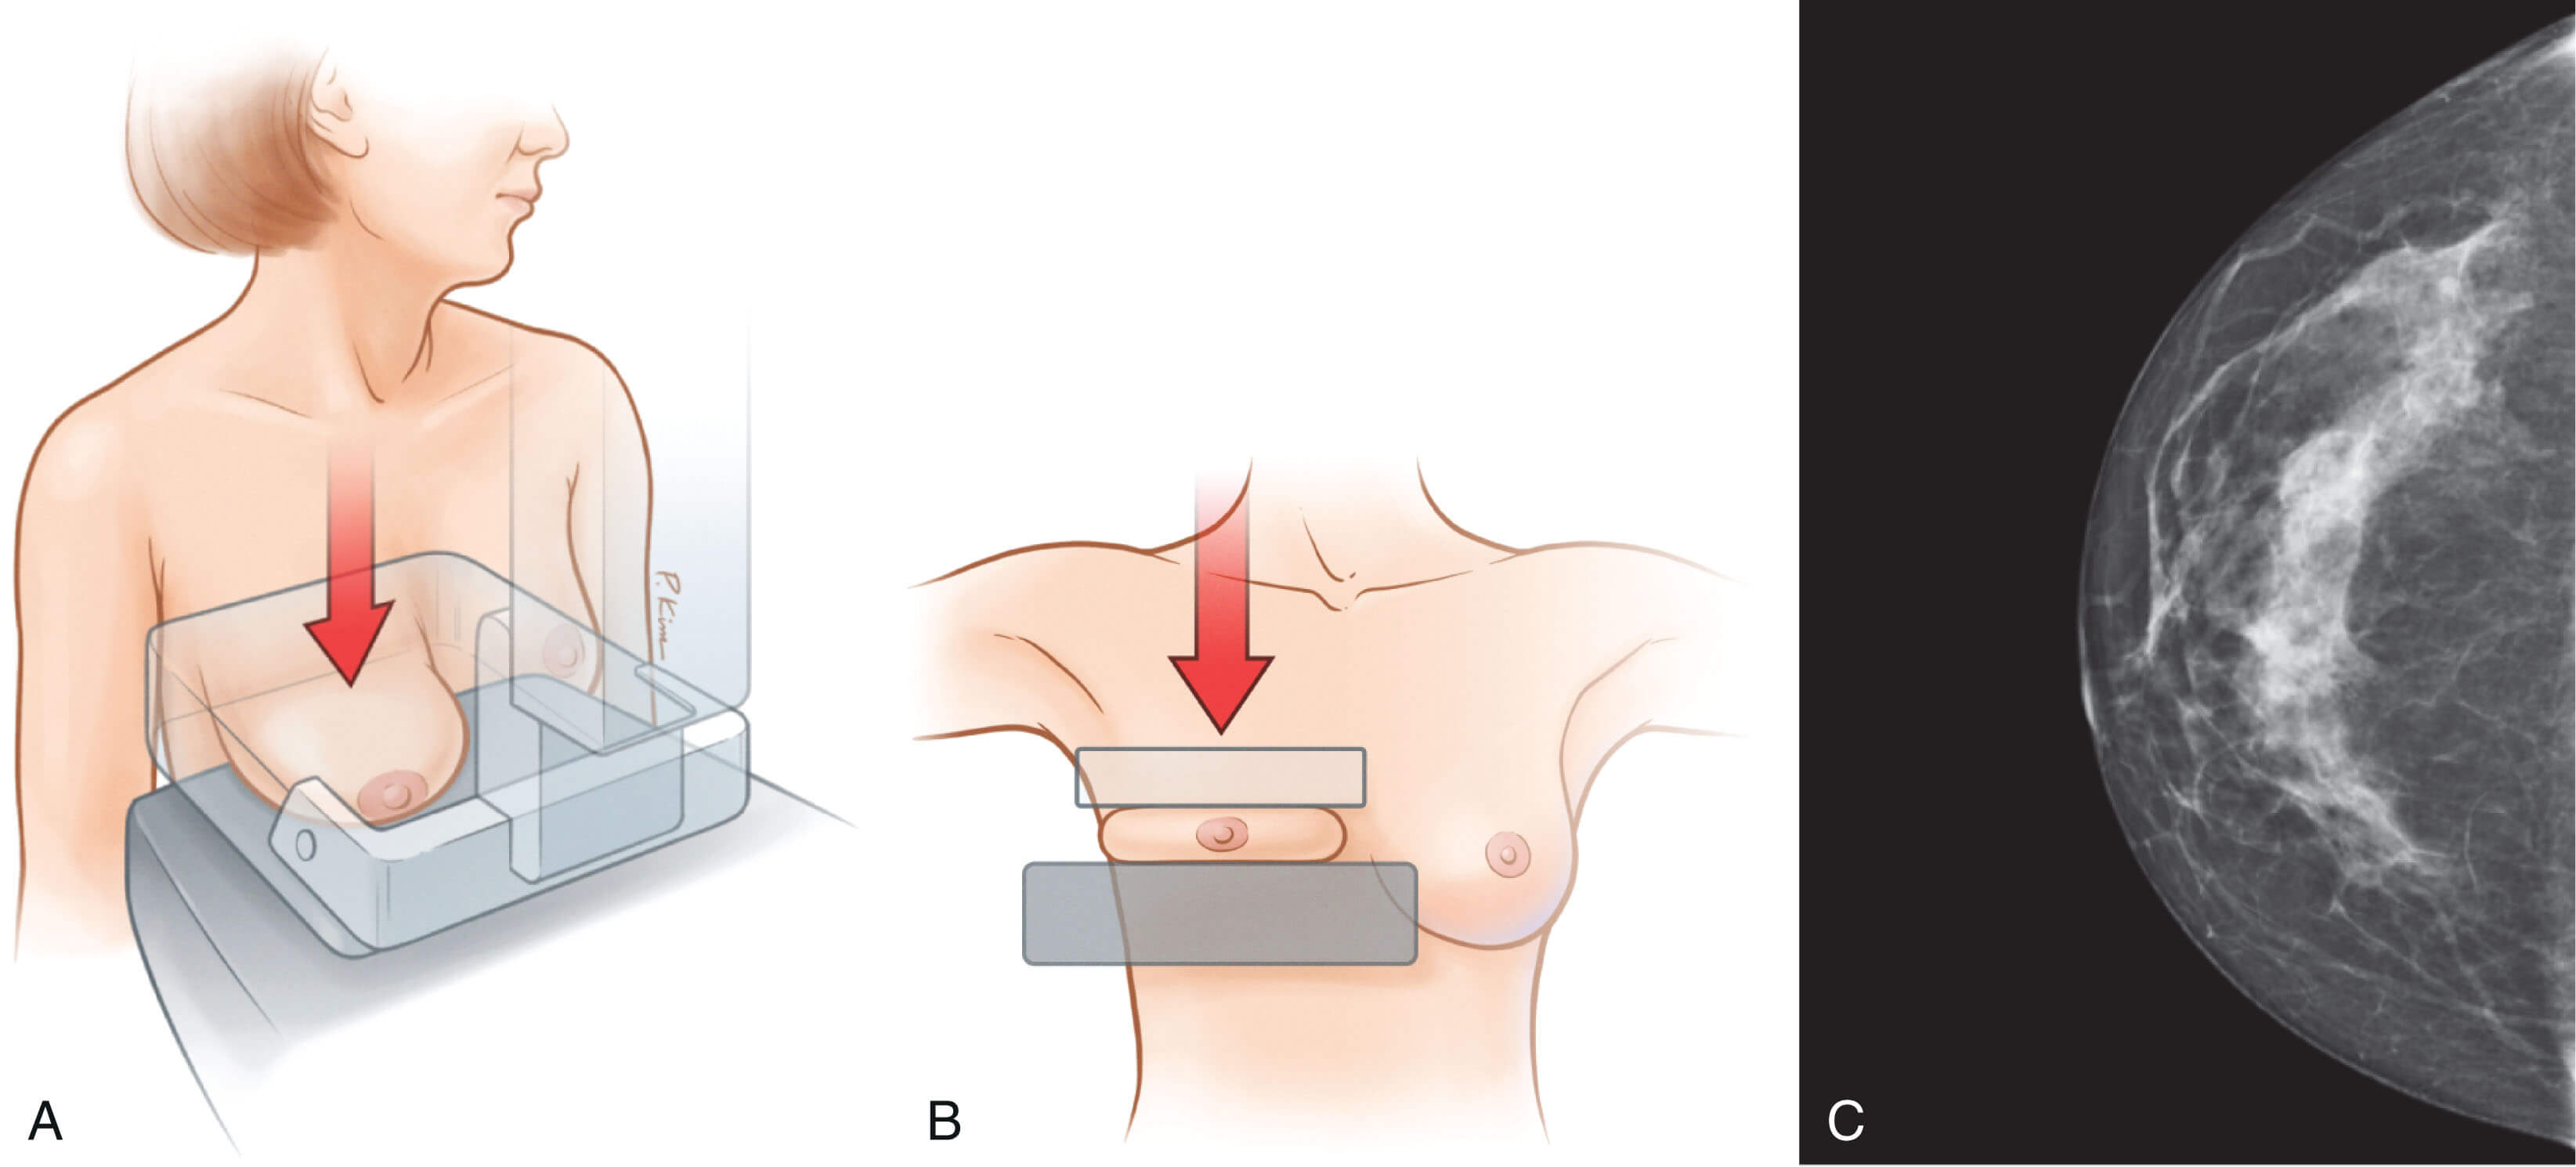
\includegraphics[width=0.6\linewidth]{reports//assets/cc_view.jpg}
    \caption[CC view acquisition procedure]{Illustration of CC view acquisition: a) The breast is positioned horizontally on the detector and compressed with a paddle. b) Top-down compression is applied to obtain the X-ray projection. 
    c) Resulting mammogram image (CC view) \cite{imaging_introduction_2022}. }
    \label{fig:cc_view}
\end{figure}

\begin{figure}[h!]
    \centering
    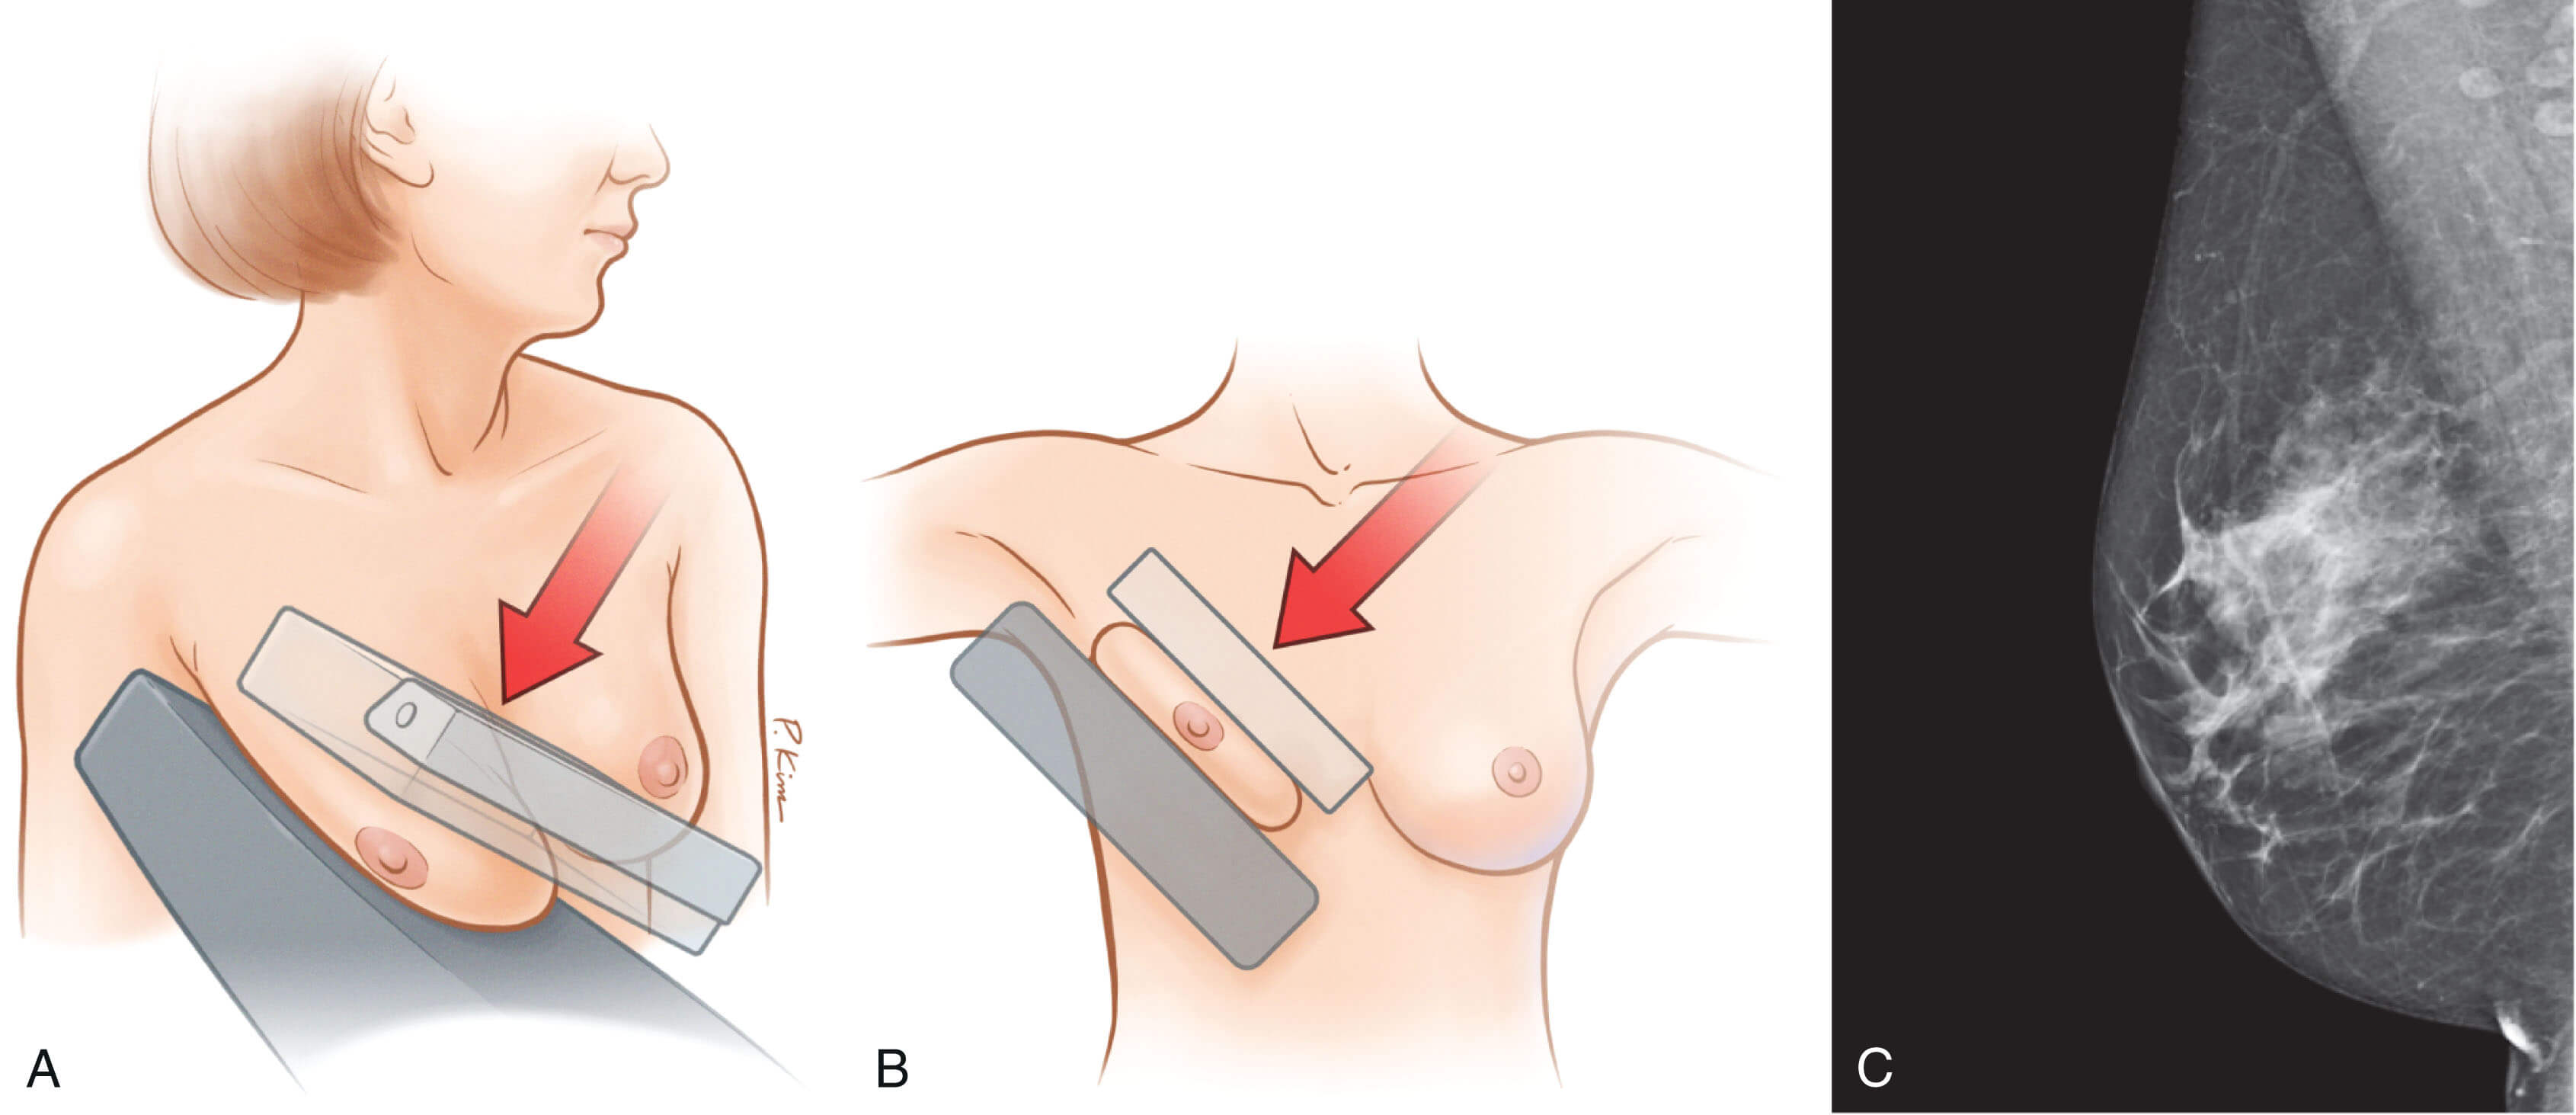
\includegraphics[width=0.6\linewidth]{reports//assets/mlo_view.jpg}
    \caption[MLO view acquisition procedure]{Illustration of MLO view acquisition: a) The breast is positioned at an oblique angle on the detector and compressed with a paddle. b) Compression is applied from the upper inner to the lower outer aspect to obtain the oblique X-ray projection. c) Resulting mammogram image (MLO view) \cite{imaging_introduction_2022}.}
    \label{fig:mlo_view}
\end{figure}


Modern mammography units can be either analog or digital, with digital mammography now representing the most widely used and preferred technology in clinical practice \cite{ltd_mammography_2025, noauthor_mammography_nodate}. Digital systems offer significant advantages over their analog counterparts, including immediate image acquisition, enhanced image quality, and easier storage and retrieval.

These technological advancements have further strengthened the role of mammography in clinical care. The use of x-ray mammography enables the identification of breast cancers, benign tumors, and cysts before they become palpable, often detecting tumors at a much earlier stage than physical examination alone \cite{staff_what_2025}. As a result, this technique is employed not only for routine screening in asymptomatic women, but also for diagnosing breast cancer following the detection of a lump or other symptoms, as well as for ongoing surveillance after a breast cancer diagnosis.

\subsection{Other modalities}

\textbf{Breast Ultrasound}

Breast ultrasound imaging is a widely used technique for breast analysis that uses a handheld device called a transducer\footnote{A device that produces sound waves that bounce off body tissues, receives the echoes, and transforms the signals into pictures.} to produce real-time images of the internal breast tissue by emitting high-frequency sound waves (Figure~\ref{fig:breast_ultrasound_comparison}).

Unlike mammography, ultrasound does not use ionizing radiation, making it a safe and non-invasive option for patients of all ages. This modality is particularly valuable for evaluating palpable lumps, distinguishing between solid and cystic masses, and further characterizing lesions detected on mammography, especially in women with dense breast tissue, where mammography may be less sensitive \cite{gokhale_ultrasound_2009}.

However, it is important to take into consideration that the accuracy and quality of ultrasound examinations are highly dependent on the skill and experience of the operator. In addition, compared to mammography, ultrasound is less effective at distinguishing between benign and malignant lesions, which may result in more follow-up procedures.

\begin{figure}[h!]
	\centering
	\begin{subfigure}[c]{0.45\textwidth}
		\centering
		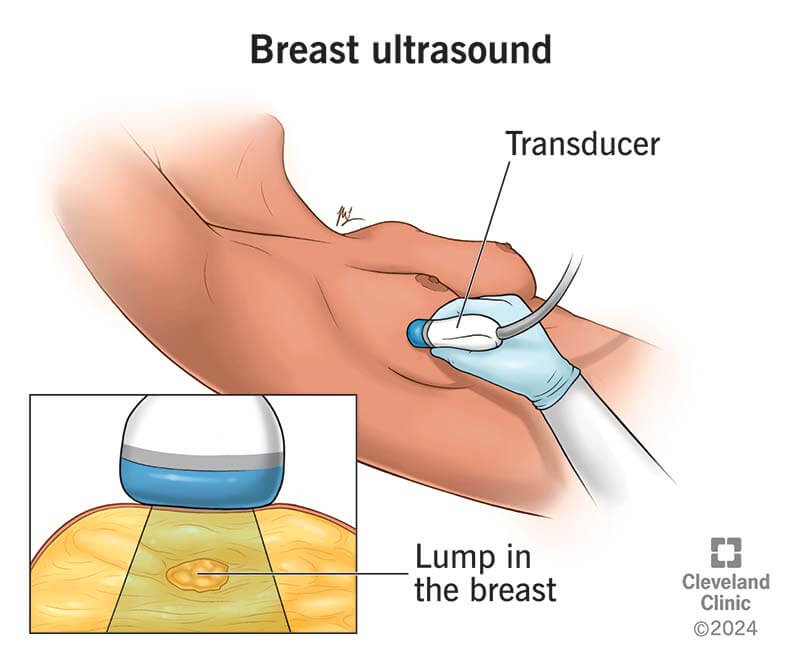
\includegraphics[width=\textwidth]{reports/assets/breast_ultrasound.jpg}
            \caption{}
		\label{fig:breast_ultrasound}
	\end{subfigure}
	\begin{subfigure}[c]{0.45\textwidth}
		\centering
		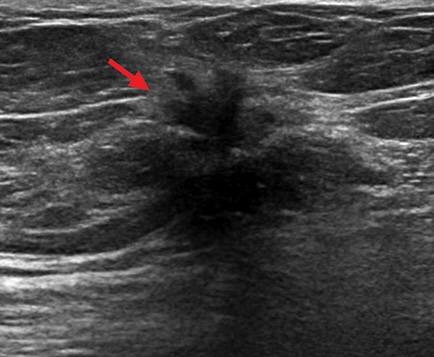
\includegraphics[width=\textwidth]{reports/assets/ultrasound.jpg}
            \caption{}
		\label{fig:ultrasound}
	\end{subfigure}
	\caption[Breast ultrasound procedure and example]{(a) Breast ultrasound representation \cite{macauley_start--finish_2022}. (b) Breast ultrasound example showing an irregular, dark gray spiculated mass, highly suspicious for cancer \cite{noauthor_breast_nodate}.}
\label{fig:breast_ultrasound_comparison}
\end{figure}

\textbf{Magnetic Resonance Imaging (MRI)}

MRI is a noninvasive imaging procedure that uses strong magnetic fields and radio waves to produce a series of highly detailed images of structures inside the body. In breast imaging, MRI operates on the same fundamental principle and is often used alongside other breast imaging modalities to detect breast cancer or other abnormalities \cite{nih_definition_2011}. 

Breast MRI is particularly valuable for women at high risk of developing breast cancer, such as those with genetic mutations or a strong family history of the disease. This is due to its high sensitivity, with detection rates exceeding 90\%, making it the most sensitive imaging modality for identifying breast cancer \cite{radswiki_breast_nodate}.

Despite these advantages, MRI is more expensive and less widely available than mammography or ultrasound. Its high sensitivity can sometimes lead to more false positives, resulting in additional follow-up imaging. Furthermore, accurate interpretation of breast MRI requires specialized training and experience \cite{noauthor_technical_nodate}.


\begin{figure}
    \centering
    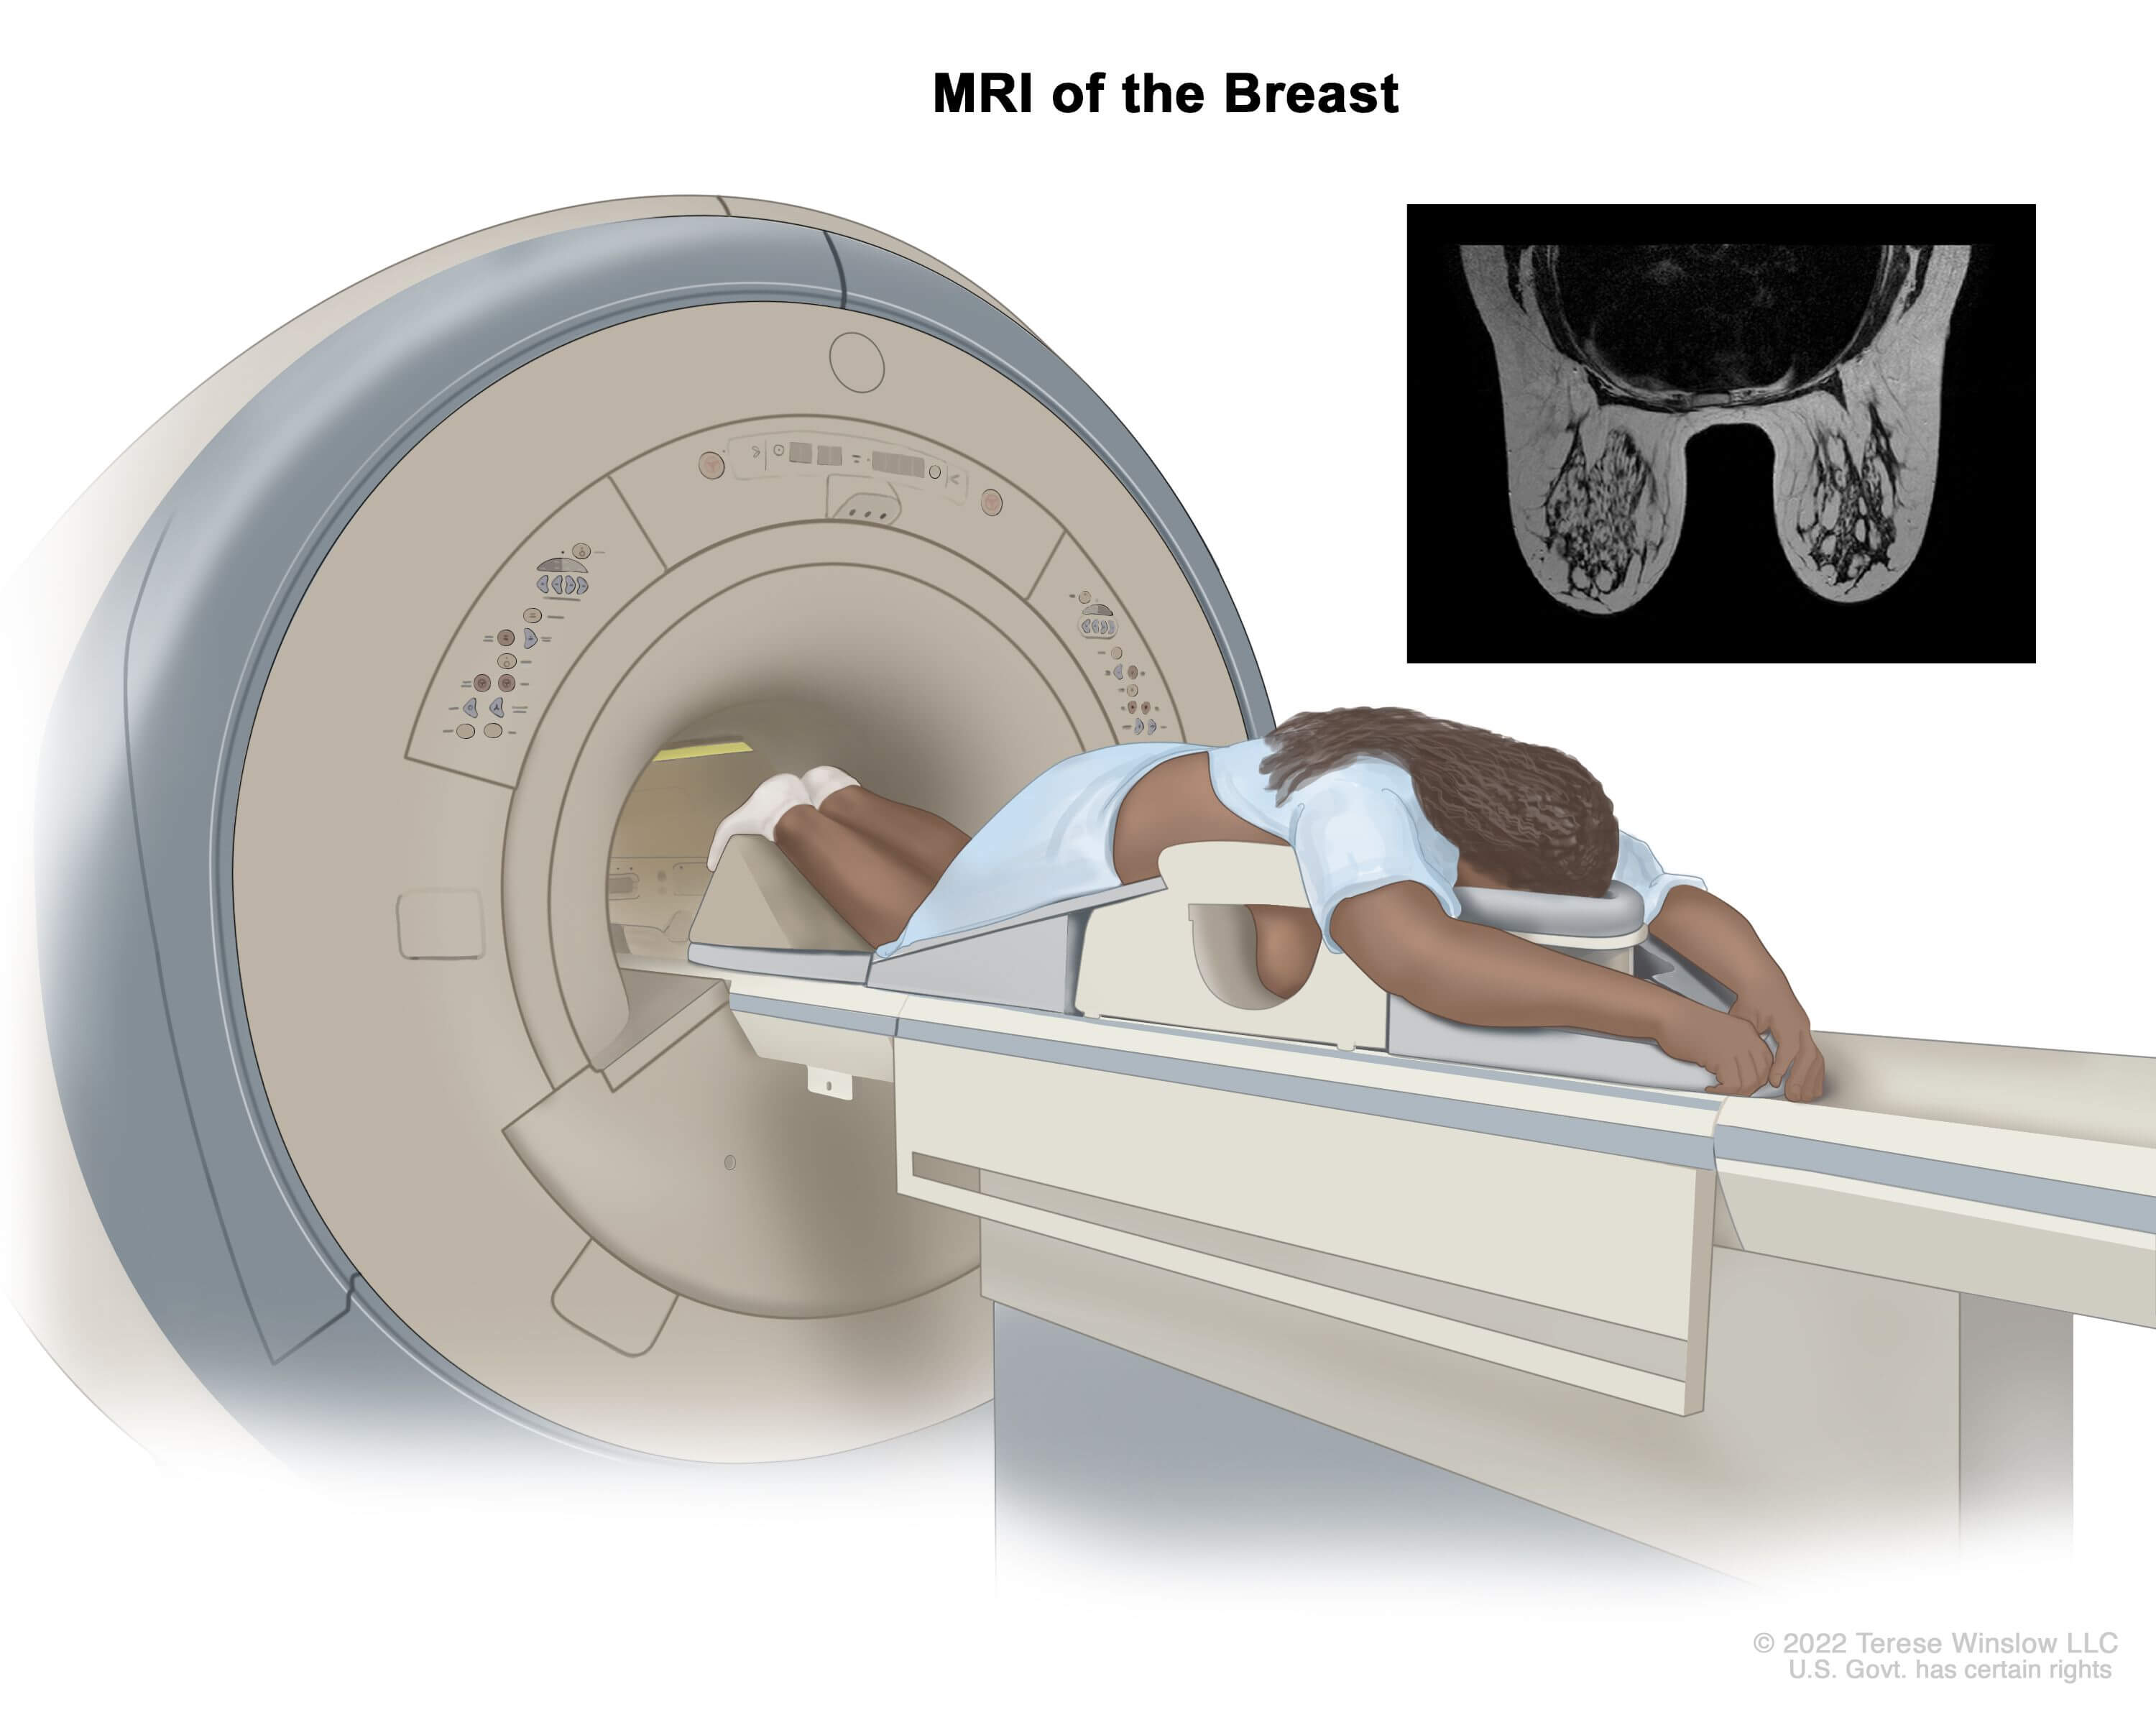
\includegraphics[width=0.5\linewidth]{reports//assets/breast_mri.jpg}
    \caption[Breast MRI procedure]{Illustration of a breast MRI procedure. The patient lies prone on a dedicated breast coil, allowing for optimal imaging of the breast tissue \cite{nih_definition_2011}.}
    \label{fig:breast_mri}
\end{figure}


\section{Cancer Screening}

Cancer screening is the process of using tests to look for cancer or pre-cancerous changes in people, mainly targeting those who do not have any symptoms of the disease. The purpose is to detect cancer at an early stage, when treatment is more likely to be successful and before symptoms appear \cite{noauthor_cancer_2010}.

There are different kinds of screening tests that can be used in the process depending on the subject’s needs. These may include physical examinations and clinical history reviews, laboratory tests, imaging procedures, and genetic tests \cite{noauthor_cancer_2010}. In the context of breast cancer, x-ray mammography is the gold-standard screening tool. As mentioned earlier, it is a widely available, noninvasive, and cost-effective technique, and it has been proven to detect tumors up to two years before they become palpable or cause symptoms \cite{cancer_que_2023}.

\subsection{General process description}

The general process of breast screening is very similar worldwide in its main steps, but certain aspects, such as the starting age, screening frequency, and technology used may vary from country to country. In Spain, the breast cancer screening program began in 1990 and is performed only in women between 50 and 69 years old, using biennial\footnote{Every two years} mammograms \cite{noauthor_ministerio_nodate}. The following steps are the core steps of breast cancer screening:

\begin{enumerate}
    \item \textbf{Invitation}: Eligible women (based on age and sometimes risk factors) are invited to participate, either through organized national programs or opportunistically via healthcare providers.
    \item \textbf{Screening test}: The screening test is performed, typically a mammogram, which may be supplemented by other tests. For example, in Spain, an ultrasound is also recommended \cite{noauthor_map_nodate}.
    \item \textbf{Image review}: Radiologists review the mammograms for signs of cancer, such as masses or microcalcifications.
    \item \textbf{Results notification}: Women are informed of their results. Those with abnormal findings are called back for additional tests.
    \item \textbf{Follow-up}: f abnormalities are detected, further diagnostic procedures, such as additional imaging or biopsy, are conducted to confirm or rule out cancer.
\end{enumerate}


At this stage, non-invasive techniques, such as those investigated in this work, can contribute to improved diagnostic outcomes and offer more detailed insights. Specifically, in the context of molecular subtype classification, having such a tool would provide additional information for cases with abnormal findings or confirmed cancers. This could lead to a better prognosis and help guide clinical decision-making, potentially reducing the need for further invasive procedures like biopsies.

\subsection{Biopsy Techniques}

When imaging or other screening tests detect abnormalities suggestive of breast cancer, a biopsy is typically required to obtain a definitive diagnosis. A breast biopsy involves removing a small sample of tissue from the suspicious area, which is then examined under a microscope by a pathologist \cite{DefinitionBiopsyNCI2011}. This step is crucial not only for confirming the presence of cancer but also for determining its type, grade, and increasingly, its molecular characteristics.

\textbf{Classification}

Several biopsy techniques are commonly used for the diagnosis and characterization of breast lesions, including:

\begin{itemize}
    \item \textbf{Fine Needle Aspiration (FNA)}: A minimally invasive procedure that uses a thin, hollow needle to extract cells or fluid from a suspicious area. It is often performed when the lesion is likely to be a cyst\footnote{A fluid-filled sac}. FNA is quick, cost-effective, and generally well-tolerated, offering high diagnostic accuracy when performed correctly. However, it may provide limited information about tissue architecture and can sometimes yield inconclusive results, necessitating further evaluation with a core needle or surgical biopsy \cite{noauthor_fine_nodate, silva_breast_2023}.
    
    \item \textbf{Core Needle Biopsy (CNB)}: This technique employs a larger, hollow needle to obtain small cylinders (cores) of tissue, usually under image guidance \cite{CoreNeedleBiopsy, silva_breast_2023}. CNB provides a more substantial tissue sample, enabling accurate histological diagnosis and molecular marker assessment-essential for molecular subtyping. It is considered the standard diagnostic approach due to its high concordance with surgical specimens for key biomarkers such as ER, PR, HER2, and Ki67 \cite{jeong_analysis_2020}.
    
    \item \textbf{Vacuum-Assisted Biopsy (VAB)}: VAB uses a vacuum-powered device to collect multiple tissue samples through a single insertion, typically guided by stereotactic or ultrasound imaging. It is particularly effective for sampling microcalcifications or small lesions detected via mammography and yields larger tissue samples, thereby reducing sampling error. This method is reliable, well-tolerated, and can sometimes eliminate the need for surgical biopsy, especially for benign lesions \cite{park_vacuum-assisted_2014}.
    
    \item \textbf{Surgical Biopsy}: When needle-based techniques are inconclusive or not feasible, a surgical biopsy may be performed to excise part or all of the suspicious tissue. While it provides the most comprehensive tissue sample, it is also more invasive and costly, and is generally reserved for cases where less invasive methods fail to yield a definitive diagnosis \cite{silva_breast_2023}.
\end{itemize}

The selection of a biopsy technique depends on factors such as lesion size, location, and imaging characteristics, as well as patient-specific considerations. Importantly, the tissue obtained through these procedures is not only used to confirm malignancy, but also to conduct immunohistochemical and molecular analyses. These analyses are essential for determining the molecular subtype of breast cancer, which, as discussed previously, plays a key role in guiding prognosis and therapeutic decision-making.

\textbf{Limitations}




\section{Artificial Intelligence in Medical Imaging}

\chapter{Technological Review}

This section explores the modern definitions and structures of AI models, as well as their use in modern medicine and specifically in medical imaging.

\section{Artificial Intelligence}

\begin{figure}[h]
    \centering
    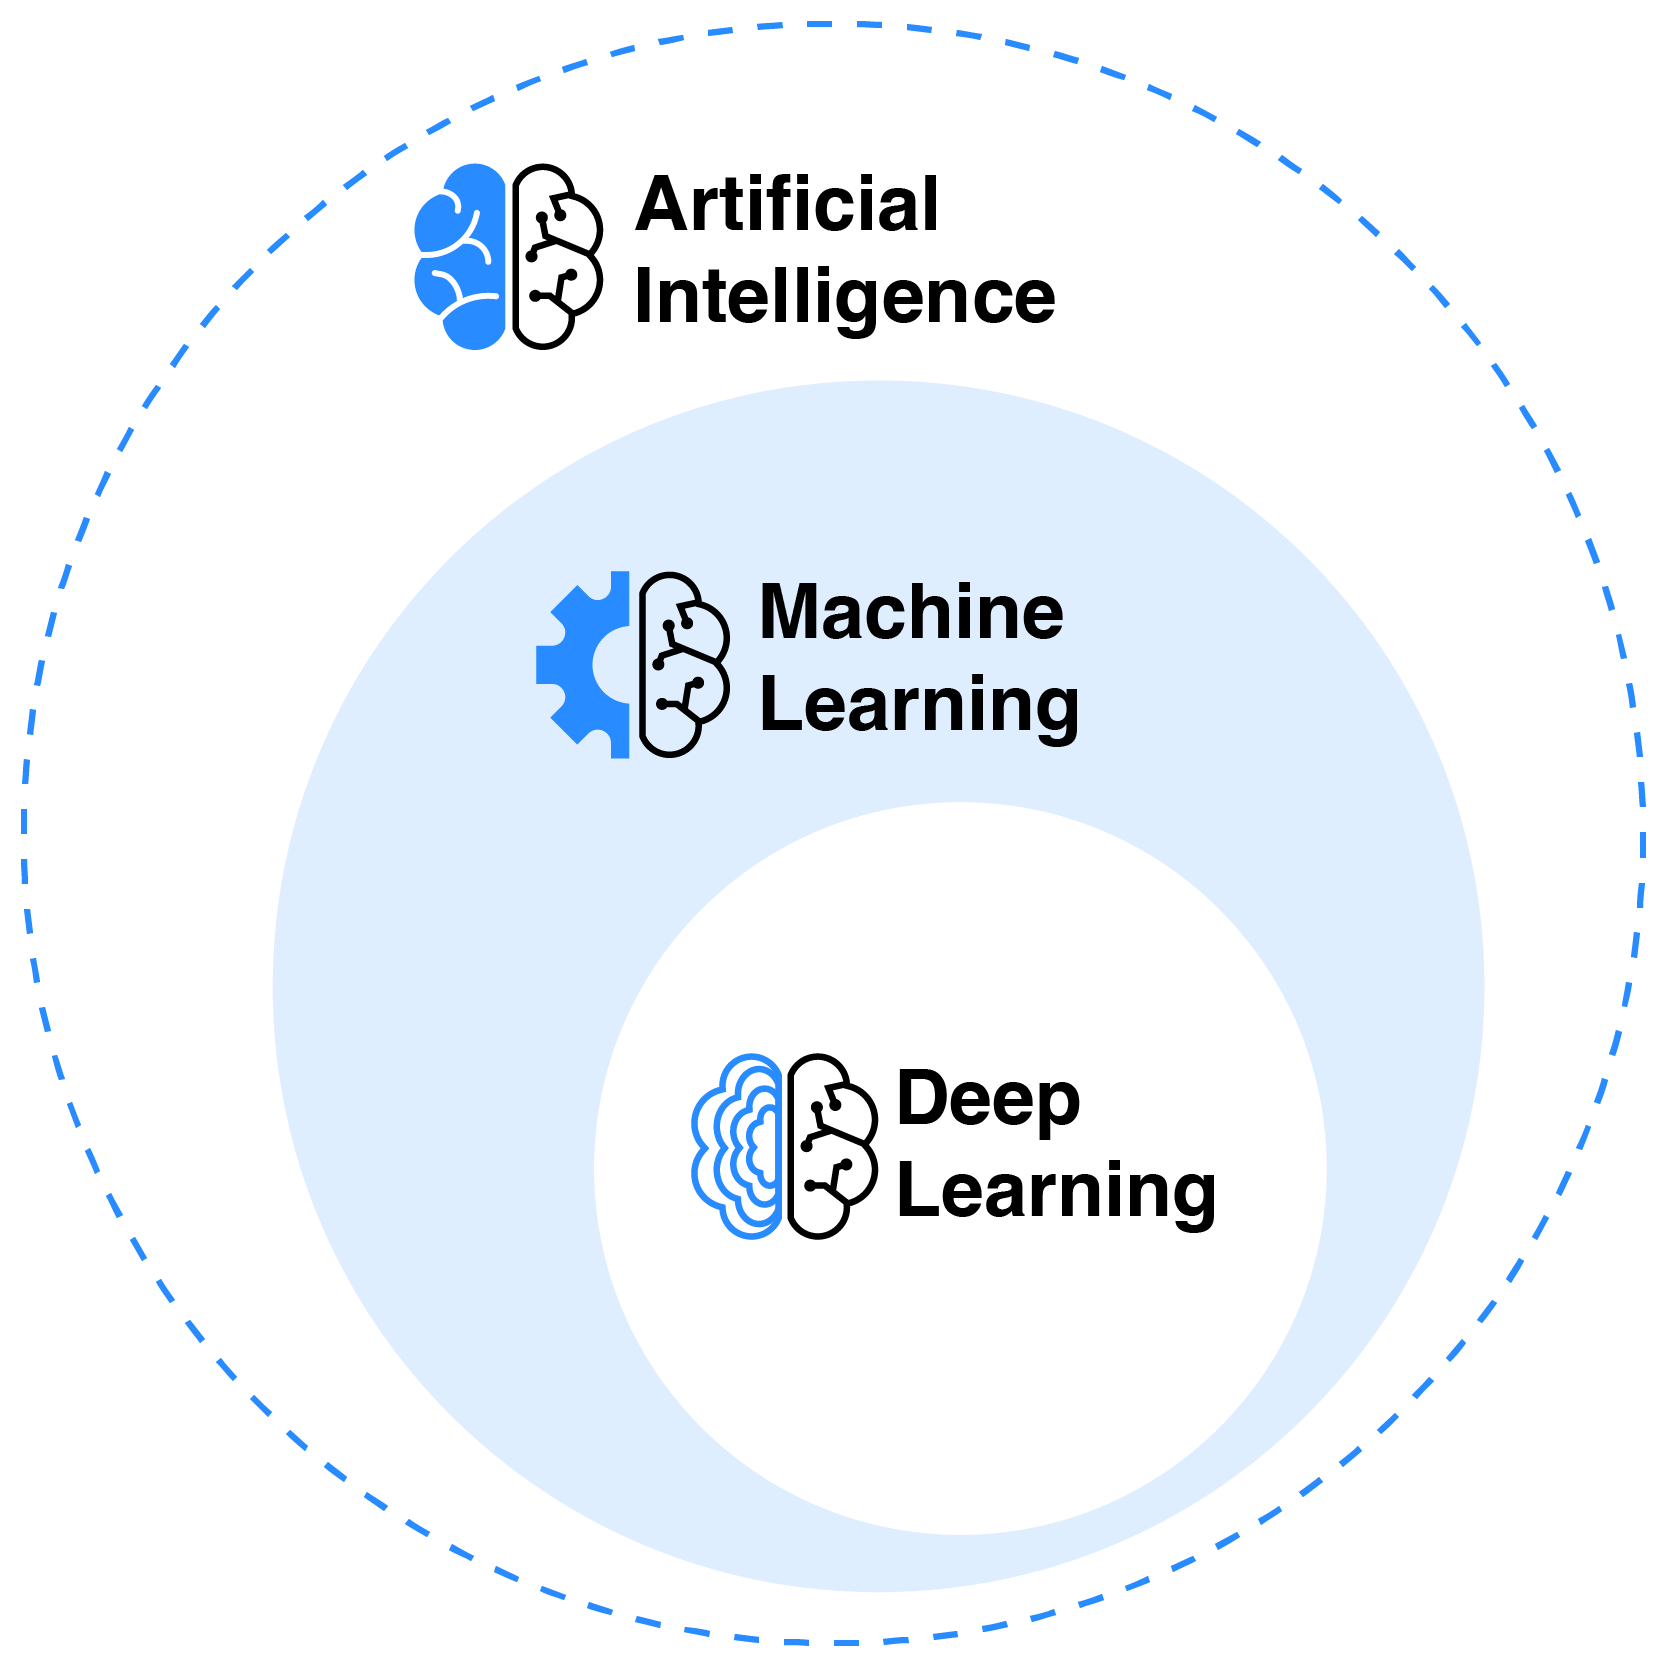
\includegraphics[width=0.5\linewidth]{reports//assets/ai.png}
    \caption[AI overview]{Complete}
    \label{fig:enter-label}
\end{figure}

\subsection{From Classical AI to Deep Learning}
\subsection{Timeline}

\section{Convolutional Neural Networks}
\subsection{General Principles}
\subsection{Historical Architectures and Variants}
\subsection{Limitations in Mammography}

\section{Vision Transformers}
\subsection{Brief History}
\subsection{Principles of Self-Attention}
\subsection{Vision Transformer (ViT)}
\subsection{Shifted-Window Transformer (Swin)}
\subsection{Multi-Axis Vision Transformer (MaxViT)}

\section{Training and Evaluation Techniques}
\subsection{Transfer Learning}
\subsection{Fine-Tuning}
\subsection{K-Fold Cross-Validation}
\chapter{Materials and Methods}

This section documents the materials and processes carried out for this study. First, the selected dataset for model training and analysis is described, followed by the processing and preparation of the images, and finally the evaluation metrics used to assess model performance.

\section{The Chinese Mammography Database}

The Chinese Mammography Database (CMMD) is a public dataset developed by Cai et al. (2023) \cite{cai_online_2023} and hosted on The Cancer Imaging Archive (TCIA)\footnote{\url{https://www.cancerimagingarchive.net/collection/cmmd/}}. This dataset includes a total of 3,712 mammograms from 1,775 Chinese patients, in craniocaudal (CC) and mediolateral oblique (MLO) views, collected between July 2012 and January 2016. CMMD is divided into two subsets: CMMD1, which contains studies with basic clinical information, and CMMD2, which also includes molecular subtype annotations. The latter is the main basis for this research, as it is the only public and freely accessible subset that provides such molecular labels explicitly. Table \ref{tab:cmmd_features} details the main characteristics of each subset.

\begin{table}
        \caption[CMMD subsets characteristics]{Main characteristics of the CMMD subsets}
	\centering
	\begin{tabular}{lccccc}
		\toprule
		                            & \textbf{CMMD1}       & \textbf{CMMD2}      &      \\
		\midrule
		\textbf{Number of patients} & 1026                 & 749                 & 1775 \\
		\textbf{Number of images}   & 2214                 & 1498                & 3712 \\
		\textbf{Mean patient age}   & 45.92 (17-84 years)  & 49.82 (21-87 years) & -    \\
		\textbf{Categories}         & Benign and Malignant & Malignant only      & -    \\
		\textbf{Molecular subtype}  & No                   & Yes                 & -    \\
		\bottomrule
	\end{tabular}
	\label{tab:cmmd_features}
\end{table}


\subsection{General Description}

As mentioned above, the focus of this study is on the CMMD2 subset. For its composition, only malignant cases with complete immunohistochemical marker information and a diagnosis of invasive carcinoma were selected, as detailed in the exclusion criteria shown in Figure \ref{fig:cmmd_criteria}. After applying these criteria, the final sample consisted of 1,498 images corresponding to 749 patients.

\begin{figure}[h]
	\centering
	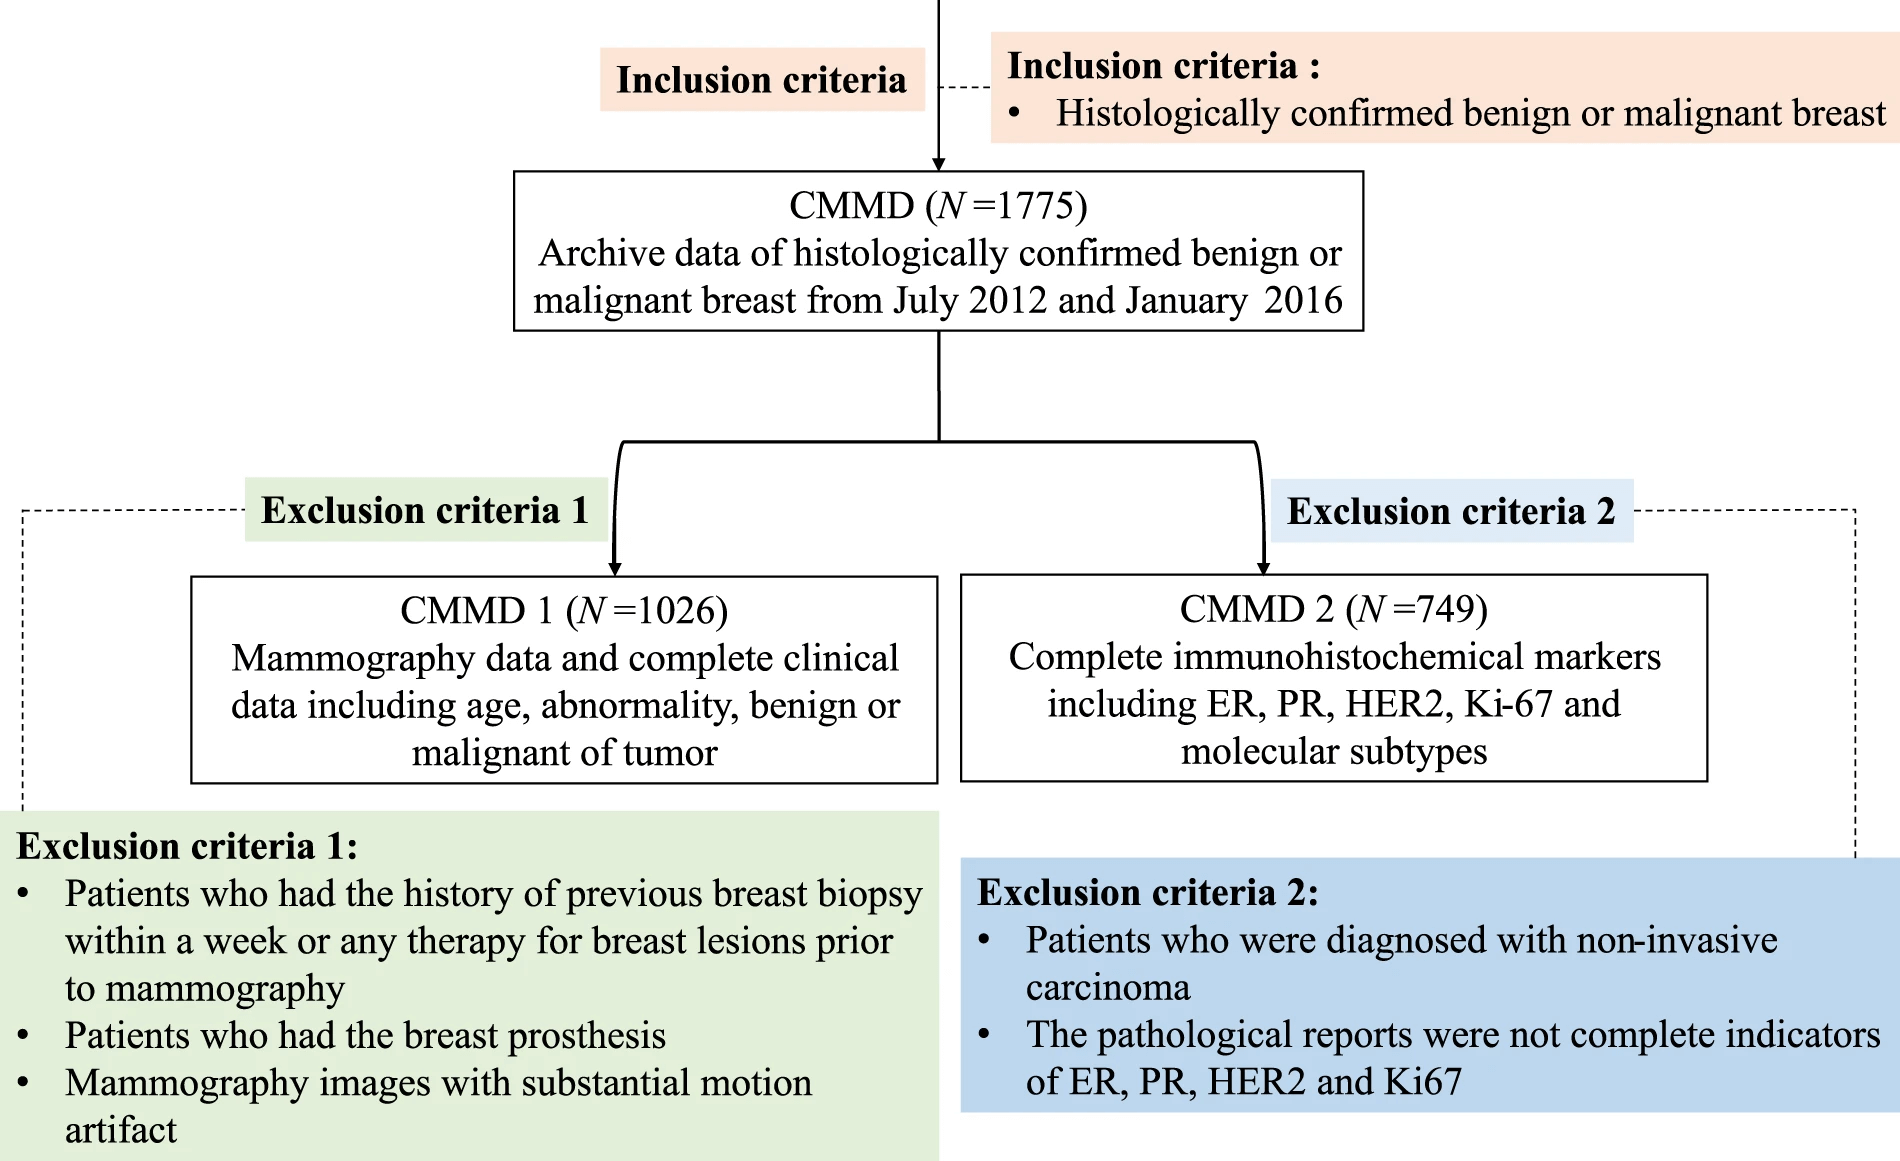
\includegraphics[width=0.8\linewidth]{reports//assets/cmmd_criteria.png}
	\caption[CMMD's inclusion and exclusion criteria]{CMMD's inclusion and exclusion criteria \cite{cai_online_2023}.}
	\label{fig:cmmd_criteria}
\end{figure}

\textbf{Image Collection}

The mammography images were collected using the \textbf{GE Senographe DS} mammography system, obtaining both CC and MLO views for each patient. The images were then stored in 8-bit grayscale at a image size of 2294×1914 pixels \cite{cai_online_2023}.

\textbf{Image Format and Resolution}

The main format of the images in the dataset is DICOM (Digital Imaging and Communications in Medicine), the standard in medical imaging, as it allows clinical metadata to be stored alongside the image and enables interoperability between equipment from different manufacturers as well as interaction between different information systems in hospitals and healthcare centers.

\newpage
\subsection{Metadata}

For each patient, the dataset provides a CSV\footnote{A plain text file that stores data in tabular form, where each line represents a row and each value in the row is separated by a comma} (Comma Separated Values) file with additional information to the obtained images, including age, laterality, type of abnormality, classification, and in the case of CMMD2, also the molecular subtype of the tumor. Table \ref{tab:cmmd2_metadata} describes these data in detail.

\begin{table}[h]
	\caption[CMMD2 metadata description]{Description of metadata variables present in the CMMD dataset.}
	\centering
	\begin{tabular}{>{\bfseries}l p{5cm} p{6cm}}
		\toprule
		\textbf{Column} & \textbf{Description}                 & \textbf{Possible values}                             \\
		\midrule
		ID1             & Unique patient identifier            & Format: D2-XXXX                                      \\
		LeftRight       & Breast laterality                    & L (left), R (right)                                  \\
		Age             & Patient age at the time of the study & Between 21 and 87 years                              \\
		Number          & Number of images available per study & Between 2 and 4                                      \\
		Abnormality     & Type of abnormality                  & Mass, Calcification, Both                            \\
		Classification  & Nature of the abnormality            & Benign, Malignant                                    \\
		Subtype         & Molecular subtype of breast cancer   & Luminal A, Luminal B, HER2-enriched, Triple negative \\
		\bottomrule
	\end{tabular}

	\label{tab:cmmd2_metadata}
\end{table}

It is important to note that, in the case of CMMD2, the laterality column indicates the side where the tumor was found; therefore, the opposite side is considered benign \cite{cai_online_2023}.

The age distribution of patients follows an approximately normal distribution with slight asymmetries. The most frequent age range is between 45 and 55 years, which is consistent with breast cancer epidemiology, where the majority of cases are diagnosed during this age interval [citation needed]. The inclusion of younger patients in the dataset enhances population diversity and enables analysis of model performance across underrepresented demographic subgroups.

\begin{figure}[h!]
	\centering
	\begin{subfigure}[c]{0.49\textwidth}
		\centering
		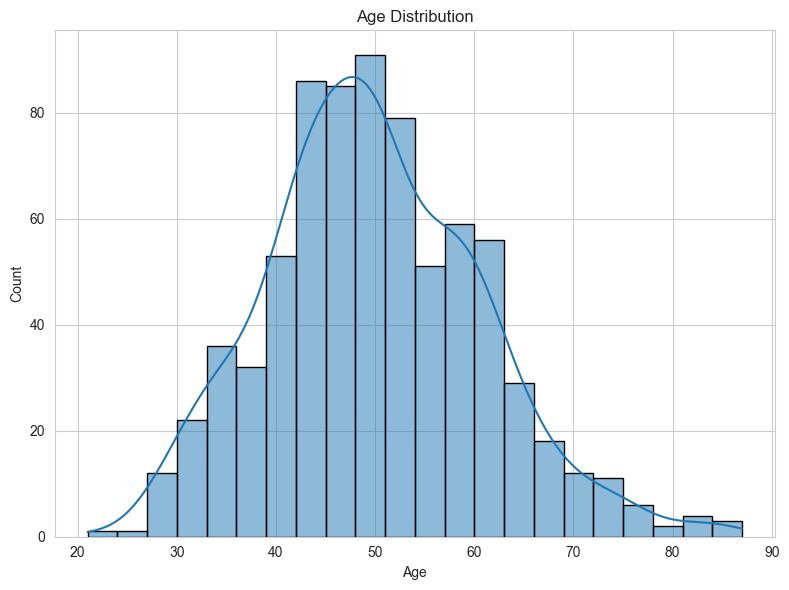
\includegraphics[width=\textwidth]{reports//assets/age.png}
		\caption{Age distribution}
		\label{fig:age_dist}
	\end{subfigure}
	\begin{subfigure}[c]{0.49\textwidth}
		\centering
		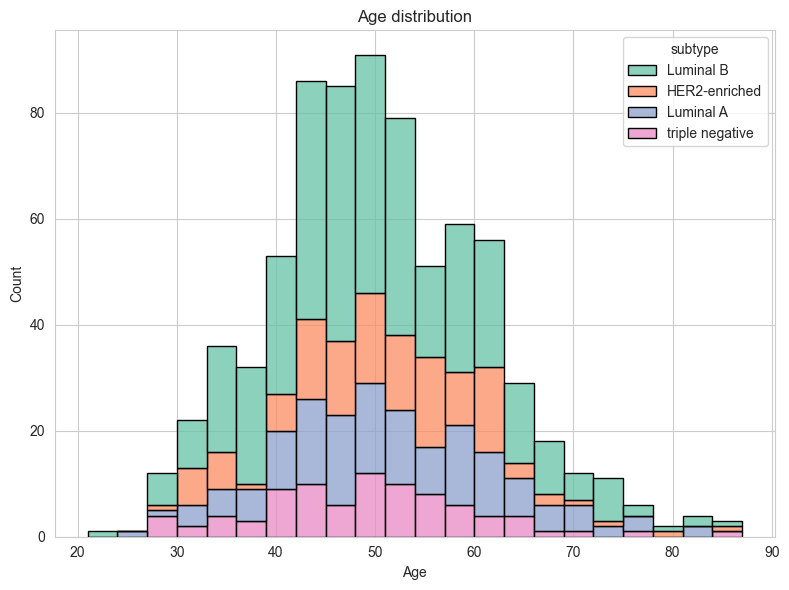
\includegraphics[width=\textwidth]{reports/assets/age_subtype.png}
		\caption{Age and subtype distribution}
		\label{fig:age_subtype}
	\end{subfigure}
	\caption[CMMD2 Age distribution]{(a) Overall age distribution of patients and (b) distribution by cancer subtype (CMMD2).}
	\label{fig:age_dist_all}
\end{figure}

Figure \ref{fig:age_dist_all} illustrates both the overall age distribution and the age distribution stratified by molecular subtype.

The analysis of molecular subtype distribution within the CMMD2 dataset is also crucial, as it determines the statistical representativeness of each class and consequently affects the models' generalization capability in clinical scenarios. The dataset exhibits significant class imbalance\footnote{Class imbalance refers to unequal representation of different classes in a dataset, where some classes have substantially more or fewer samples than others.}, with Luminal B being the most prevalent subtype (376 patients, 50.2\%), followed by Luminal A (152 patients, 20.3\%), HER2-enriched (135 patients, 18.0\%), and Triple Negative as the least represented subtype (86 patients, 11.5\%).

The class imbalance is also reflected in the total number of images available per subtype, as each patient contributes at least two mammographic views (CC and MLO projections), with few exceptions. This imbalance presents a significant challenge for machine learning classification models, which tend to exhibit bias toward majority classes when appropriate balancing strategies are not implemented. Nevertheless, this distribution accurately reflects the relative prevalence observed in clinical practice, where Luminal subtypes (A and B) are most common, while Triple Negative breast cancer represents approximately 10-15\% of all cases.

\begin{figure}[h!]
	\centering
	\begin{subfigure}[c]{0.45\textwidth}
		\centering
		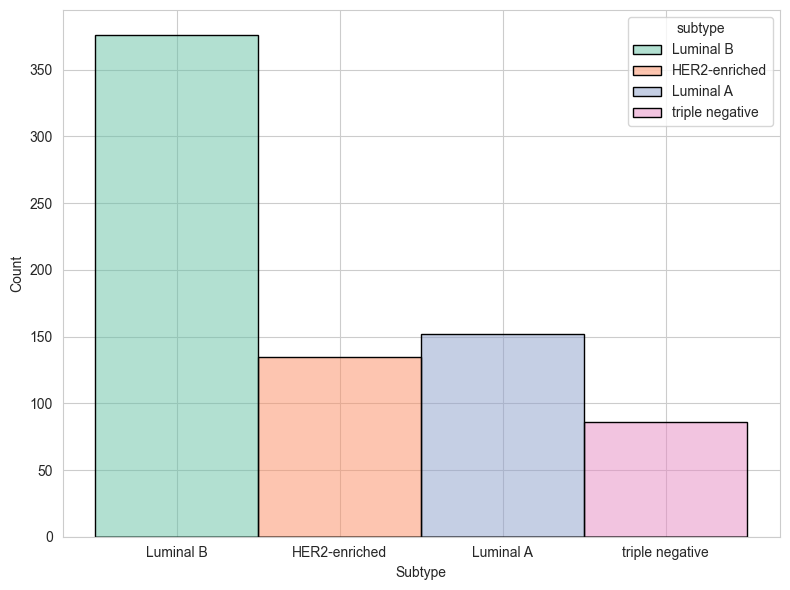
\includegraphics[width=\textwidth]{reports//assets/subtype_hist.png}
		\caption{Subtype distribution}
		\label{fig:subtype_hist}
	\end{subfigure}
	\begin{subfigure}[c]{0.45\textwidth}
		\centering
		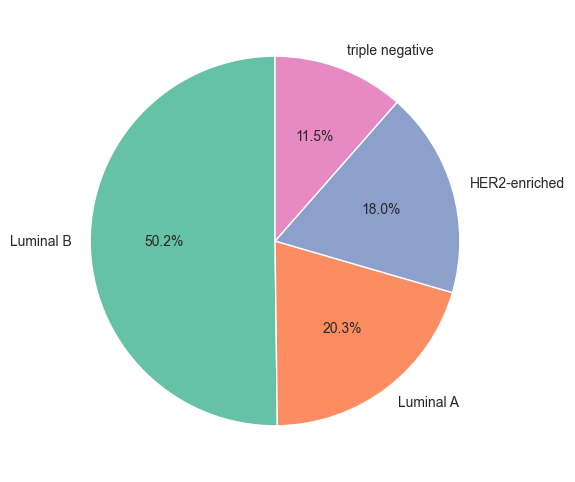
\includegraphics[width=\textwidth]{reports/assets/subtype_pie.png}
		\caption{Subtype distribution (pie chart)}
		\label{fig:subtype_pie}
	\end{subfigure}
	\caption[CMMD2 molecular subtypes distribution]{Subtype distribution of patients (CMMD2)}
	\label{fig:subtype_charts}
\end{figure}


\begin{figure}[h!]
	\centering
	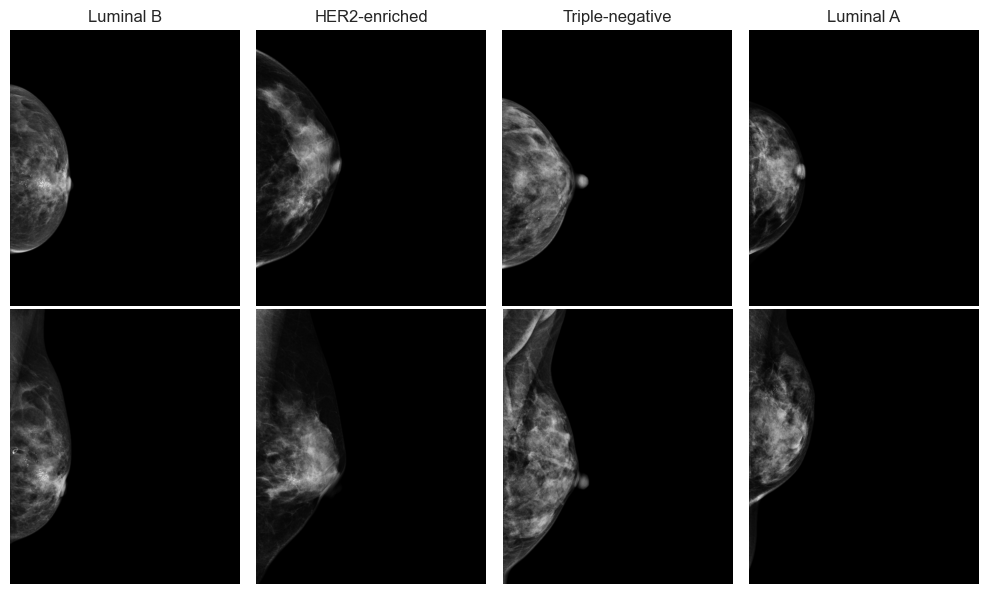
\includegraphics[width=1\linewidth]{reports//assets/images_examples.png}
	\caption[CMMD2 mammography images examples]{Example of mammography images of the CCMD2 dataset. Top row represent a CC view whereas bottom row illustrated a MLO view. Each column depicted one subtype of cancer.}
	\label{fig:cmmd-examples}
\end{figure}

\newpage
\section{The TOMPEI-CMMD Dataset review}

The TOMPEI-CMMD dataset represents an enhanced version of the original CMMD, developed by Kashiwada et al. (2025) \cite{kashiwada_tompei-cmmd_2025}. This enhancement aimed to provide comprehensive radiological insights and perform a systematic re-evaluation of the existing mammographic images. A board-certified radiologist with 20 years of experience in breast imaging assessed all images, documenting detailed radiological findings including masses, calcifications, focal asymmetric densities, architectural distortions, and their anatomical locations. The dataset further provides pixel-level segmentation masks for all identified findings in MLO views, created following the radiologist's expert assessment. 

One of the most important results of the evaluation process was the exclusion of 140 breast images that did not meet the quality and diagnostic criteria. 

\section{Image Preprocessing}
\section{Data splitting and stratification strategy}
\section{Experiments}

\section{Evaluation Metrics}

\chapter{Results and Discussion}
\section{Results}

\chapter{Conclusions and Future Work}

%%%%%%%%%%%%%%%%%%%%%%%%%%%%%%%%%%%%%%%%%%%%%%%%%%%%%%%%%%%%%%%%%%%%%%%%%
\backmatter
\selectlanguage{english}
\addcontentsline{toc}{chapter}{Bibliography}
\bibliographystyle{IEEEtran}
\bibliography{references}

\end{document}